%%%%%%%%%%%%%%%%%%%%%%%%%%%%%%%%%%%%%%%%%%%%%%%%%%%%%%%%%%%%%%%%%%%%%%%%%%%%%%%

\documentclass[12pt,twocolumn,tighten]{aastex63}
%\documentclass[12pt,twocolumn,tighten,trackchanges]{aastex63}
\usepackage{amsmath,amstext,amssymb}
\usepackage[T1]{fontenc}
\usepackage{apjfonts}
\usepackage[figure,figure*]{hypcap}
\usepackage{graphics,graphicx}
\usepackage{hyperref}
\usepackage{natbib}
\usepackage[caption=false]{subfig} % for subfloat
\usepackage{enumitem} % for specific spacing of enumerate
\usepackage{epigraph}

\renewcommand*{\sectionautorefname}{Section} %for \autoref
\renewcommand*{\subsectionautorefname}{Section} %for \autoref

\newcommand{\cn}{NGC\,2516} % cluster name

% gaia target sample numbers
\newcommand{\nkinematic}{3{,}298\ } % "fullfaint" kinematic sample, core+halo (CG18+KC19+M21). from any call of earhat.helpers._get_fullfaint_dataframes
\newcommand{\nnbhd}{13{,}843\ } % make_compstar_NGC_2516_sourcelist.py
\newcommand{\ncore}{1{,}106}  % "fullfaint" kinematic sample, CG18. from any call of earhat.helpers._get_fullfaint_dataframes
\newcommand{\nhalo}{2{,}2192} % "fullfaint" kinematic sample, KC19+M21. from any call of earhat.helpers._get_fullfaint_dataframes

% from drivers.cluster_rotation.get_auto_rotation_periods.py;  checked with plot_target_vs_actual_list_sanity_checks.py
\newcommand{\ncdips}{2{,}205\ }
\newcommand{\nkinematicrpltsixteen}{2{,}270\ }
\newcommand{\nkinematicCGandKC}{2{,}236\ }

% cdips results numbers
\newcommand{\numcdipslcs}{671{,}901\ } % drivers.yield_calculation.count_cdips_lcs.py; 2021.01.13
\newcommand{\numsouthernuniqlcs}{483{,}407\ } % drivers.yield_calculation.count_cdips_lcs.py; 2021.01.13

\newcommand{\ncalibration}{9{,}619{,}784\ } % /nfs/phtess2/ar0/TESS/PROJ/lbouma/CDIPS_LCS/counts/check_sum, 2021.02.02
\newcommand{\nnbhdcaliblc}{9{,}790\ } % get_auto_rotation_periods.py
\newcommand{\nnbhdcalibstar}{1{,}987\ } % get_auto_rotation_periods.py

\newcommand{\nautorotdenominator}{1{,}641\ } % plot_autorotation.py, w/ runid=NGC_2516. For nequal<=0, nclose<=1, LSP>0.08. See /doc/20210205_nequal_and_Prot_vs_color_cleanup.txt
\newcommand{\nautorotnumerator}{987\ } % plot_autorotation.py, For nequal<=0, nclose<=1, LSP>0.08. See /doc/20210205_nequal_and_Prot_vs_color_cleanup.txt
\newcommand{\nautorotnumeratormatching}{507\ } % plot_autorotation.py, LSP=SPDM period
\newcommand{\ncompstardenominator}{820\ } % plot_autorotation.py, w/ runid=compstar_NGC_2516. For nequal<=0, nclose<=1, LSP>0.08. 
\newcommand{\ncompstarnumerator}{365\ } % plot_autorotation.py
\newcommand{\ncompfrac}{44.5\%} % plot_autorotation.py
\newcommand{\nautovscompstardenominator}{705\ } % plot_autorotation.py, w/ runid=compstar_NGC_2516. For nequal<=0, nclose<=1, LSP>0.08. 
\newcommand{\nautovscompstarnumerator}{374\ } % plot_autorotation.py
\newcommand{\nautofrac}{53.1\%} % plot_autorotation.py

\newcommand{\kms}{\,km\,s$^{-1}$}

%% Reintroduced the \received and \accepted commands from AASTeX v5.2.
%% Add "Submitted to " argument.
\received{---}
\revised{---}
\accepted{---}
\submitjournal{ApJL.}
\shorttitle{Core \& Halo of NGC\,2516}

\begin{document}

\defcitealias{bouma_wasp4b_2019}{B19}
\defcitealias{cantatgaudin_gaia_2018}{CG18}
\defcitealias{kounkel_untangling_2019}{KC19}
\defcitealias{meingast_2021}{M21}

\title{
  Cluster Difference Imaging Photometric Survey. III.
  %The Coeval Core \& Halo of NGC\,2516
  %The Halo of NGC\,2516 Extends To At Least 300\,pc
  An Open Cluster With a 300\,pc Halo
  %NGC\,2516  300\,pc
}

%\suppressAffiliations
%\NewPageAfterKeywords
\correspondingauthor{L.\,G.\,Bouma}
\email{luke@astro.princeton.edu}

%
% key contributions
%
\author[0000-0002-0514-5538]{L. G. Bouma}
\affiliation{Department of Astrophysical Sciences, Princeton University, 4 Ivy Lane, Princeton, NJ 08540, USA}

\author[0000-0001-8732-6166]{J. D. Hartman}
\affiliation{Department of Astrophysical Sciences, Princeton University, 4 Ivy Lane, Princeton, NJ 08540, USA}

% PENDING
\author[0000-0001-7409-5688]{G. Stefansson} % halpha, bisectors, spec analysis
\affiliation{Department of Astrophysical Sciences, Princeton University, 4 Ivy Lane, Princeton, NJ 08540, USA}

%PENDING
\author[0000-0002-4891-3517]{G. Zhou} % metallicity analysis++
\affiliation{Center for Astrophysics \textbar \ Harvard \& Smithsonian, 60 Garden St, Cambridge, MA 02138, USA}

%PENDING
\author[0000-0002-9158-7315]{R. Brahm} %rafael.brahm@uai.cl coordination, WINE board
\affiliation{Facultad de Ingenier\'{i}a y Ciencias, Universidad Adolfo Ib\'a\~nez, Av.\ Diagonal las Torres 2640, Pe\~nalol\'en, Santiago, Chile}
\affiliation{Millennium Institute for Astrophysics, Chile}

%PENDING
\author[0000-0002-5674-2404]{P. Evans}
\affiliation{El Sauce Observatory, Coquimbo Province, Chile}

%PENDING
\author[0000-0001-6588-9574]{K. A. Collins} % karenacollins@outlook.com
\affiliation{Center for Astrophysics \textbar \ Harvard \& Smithsonian, 60 Garden St, Cambridge, MA 02138, USA}

%PENDING
\author[0000-0001-8045-1765]{E. Flowers}
\affiliation{Department of Astrophysical Sciences, Princeton University, 4 Ivy Lane, Princeton, NJ 08540, USA}

%PENDING
\author[0000-0002-8964-8377]{S. N. Quinn} % squinn@cfa.harvard.edu, CHIRON vetting spectrum
\affiliation{Center for Astrophysics \textbar \ Harvard \& Smithsonian, 60 Garden St, Cambridge, MA 02138, USA}

% %PENDING
% \author{J. de Leon}
% \affiliation{Department of Astronomy, University of Tokyo, 7-3-1 Hongo, Bunkyo-ky, Tokyo 113-0033, Japan}
% 
% %PENDING
% \author[0000-0002-4881-3620]{J. Livingston}
% \affiliation{Department of Astronomy, University of Tokyo, 7-3-1 Hongo, Bunkyo-ky, Tokyo 113-0033, Japan}
%
% %PENDING
% \author[0000-0003-2989-7774]{C. Bergmann}
% \affiliation{Exoplanetary Science at UNSW, School of Physics, UNSW Sydney, NSW 2052, Australia}
% \affiliation{Deutsches Zentrum f\"ur Luft- und Raumfahrt, M\"unchener Str. 20, 82234 Wessling, Germany}

%PENDING
\author[0000-0002-3481-9052]{K. G. Stassun}
\affiliation{Vanderbilt University, Department of Physics \& Astronomy, 6301 Stevenson Center Lane, Nashville, TN 37235, USA}
\affiliation{Fisk University, Department of Physics, 1000 17th Avenue N., Nashville, TN 37208, USA}
%

%
% Princeton team
%
%PENDING
\author[0000-0002-0628-0088]{W. Bhatti}
\affiliation{Department of Astrophysical Sciences, Princeton University, 4 Ivy Lane, Princeton, NJ 08540, USA}
%
\author[0000-0002-4265-047X]{J. N. Winn}
\affiliation{Department of Astrophysical Sciences, Princeton University, 4 Ivy Lane, Princeton, NJ 08540, USA}
%
\author[0000-0001-7204-6727]{G. \'A. Bakos}
\affiliation{Department of Astrophysical Sciences, Princeton University, 4 Ivy Lane, Princeton, NJ 08540, USA}

%
% SG1 contributors
%

% % begin (ASTEP team)
% %PENDING
% \author{L. Abe} % Lyu
% \affiliation{Universit\'e C\^{o}te d'Azur, Observatoire de la C\^ote d'Azur, CNRS, Laboratoire Lagrange, Bd de l'Observatoire, CS 34229, 06304 Nice cedex 4, France}
% 
% %%PENDING->OMITTED
% %\author{A. Agabi} % Abdelkrim 
% %\affiliation{Universit\'e C\^{o}te d'Azur, Observatoire de la C\^ote d'Azur, CNRS, Laboratoire Lagrange, Bd de l'Observatoire, CS 34229, 06304 Nice cedex 4, France}
% 
% %PENDING
% \author[0000-0001-7866-8738]{N. Crouzet} % Nicolas
% \affiliation{European Space Agency, European Space Research and Technology Centre (ESA/ESTEC), Keplerlaan 1, 2201 AZ Noordwijk, The Netherlands}
% 
% %PENDING
% \author[0000-0002-3937-630X]{G. Dransfield} % Georgina
% \affiliation{School of Physics \& Astronomy, University of Birmingham, Edgbaston, Birmingham B15 2TT, United Kingdom}
% 
% \author[0000-0002-7188-8428]{T. Guillot} % Tristan 
% \affiliation{Universit\'e C\^{o}te d'Azur, Observatoire de la C\^ote d'Azur, CNRS, Laboratoire Lagrange, Bd de l'Observatoire, CS 34229, 06304 Nice cedex 4, France}
% 
% %PENDING
% \author{W. Marie-Sainte} % Wenceslas
% \affiliation{Institut Paul \'{E}mile Victor, Concordia Station, Antarctica}
% 
% %PENDING
% \author{D. M\'ekarnia} % Djamel
% \affiliation{Universit\'e C\^{o}te d'Azur, Observatoire de la C\^ote d'Azur, CNRS, Laboratoire Lagrange, Bd de l'Observatoire, CS 34229, 06304 Nice cedex 4, France}
% 
% %PENDING
% \author[0000-0002-5510-8751]{A. H.M.J. Triaud} % Amaury
% \affiliation{School of Physics \& Astronomy, University of Birmingham, Edgbaston, Birmingham B15 2TT, United Kingdom}
% % end (ASTEP team)

%
% SG2/SG3 contributors
%
\author{J.~Teske} % PFS
\affiliation{Earth and Planets Laboratory, Carnegie Institution for Science, 5241 Broad Branch Road, NW, Washington, DC 20015, USA}

\author{S.~X.~Wang}% PFS
\affiliation{Department of Astronomy, Tsinghua University, Beijing 100084, People's Republic of China}

\author{R. P. Butler}% PFS
\affiliation{Earth and Planets Laboratory, Carnegie Institution for Science, 5241 Broad Branch Road, NW, Washington, DC 20015, USA}

\author{J. D. Crane}% PFS
\affiliation{Observatories of the Carnegie Institution for Science, 813 Santa Barbara Street, Pasadena, CA 91101, USA}

\author{S. A. Shectman}% PFS
\affiliation{Observatories of the Carnegie Institution for Science, 813 Santa Barbara Street, Pasadena, CA 91101, USA}



% %PENDING
% \author[0000-0002-7595-0970]{C.~G.~Tinney}
% \affiliation{Exoplanetary Science at UNSW, School of Physics, UNSW Sydney, NSW 2052, Australia}


% %
% % WINE MPIA team
% %
% 
% %PENDING
% \author{T. Henning} %Thomas henning@mpia.de FEROS, WINE board
% \affiliation{Max-Planck-Institut f\"{u}r Astronomie, K\"onigstuhl 17, Heidelberg 69117, Germany }
% 
% %PENDING
% \author[0000-0001-9513-1449]{N. Espinoza} %N\'estor nespinoza@stsci.edu WINE board
% \affiliation{Space Telescope Science Institute, 3700 San Martin Drive, Baltimore, MD 21218, USA}
% 
% %PENDING
% \author[0000-0002-5389-3944]{A. Jord\'an} %andres.jordan@gmail.com WINE board
% \affiliation{Facultad de Ingenier\'{i}a y Ciencias, Universidad Adolfo Ib\'a\~nez, Av.\ Diagonal las Torres 2640, Pe\~nalol\'en, Santiago, Chile}
% \affiliation{Millennium Institute for Astrophysics, Chile}
% 
% %PENDING
% \author{M. Barbieri} %Maruo mauro.barbieri@uda.cl FEROS observations
% \affiliation{INCT, Universidad de Atacama, calle Copayapu 485, Copiap\'o, Atacama, Chile}
% 
% %PENDING
% \author{S. Nandakumar} %sangeetha.nandakumar@postgrados.uda.cl  FEROS observations
% \affiliation{INCT, Universidad de Atacama, calle Copayapu 485, Copiap\'o, Atacama, Chile}
% 
% %PENDING
% \author{T. Trifonov} %Trifon trifonov@mpia.de FEROS observations
% \affiliation{Max-Planck-Institut f\"{u}r Astronomie, K\"onigstuhl 17, Heidelberg 69117, Germany }
% 
% %PENDING
% \author[0000-0002-1896-2377]{J.~I.~Vines} %Jose jose.vines.l@gmail.com FEROS observations
% \affiliation{Departamento de Astronom\'ia, Universidad de Chile, Camino El Observatorio 1515, Las Condes, Santiago, Chile}
% 
% %PENDING
% \author{M. Vuckovic} %Maja maja.vuckovic@uv.cl FEROS observations
% \affiliation{Instituto de F\'isica y Astronom\'ia, Universidad de Vapara\'iso, Casilla 5030, Valpara\'iso, Chile}

%
% SG4 contributors
%
%PENDING
\author[0000-0002-0619-7639]{C.~Ziegler} % carl.ziegler@dunlap.utoronto.ca
\affiliation{Dunlap Institute for Astronomy and Astrophysics, University of Toronto, 50 St. George Street, Toronto, Ontario M5S 3H4, Canada}

%%OMITTED
%\author{C.~Brice\~{n}o} % cbriceno@ctio.noao.edu
%\affiliation{Cerro Tololo Inter-American Observatory, Casilla 603, La Serena, Chile}

%PENDING
\author{N.~Law} % nlaw@unc.edu
\affiliation{Department of Physics and Astronomy, The University of North Carolina at Chapel Hill, Chapel Hill, NC 27599-3255, USA}

%PENDING
\author[0000-0003-3654-1602]{A.~W.~Mann} % awmann@unc.edu
\affiliation{Department of Physics and Astronomy, The University of North Carolina at Chapel Hill, Chapel Hill, NC 27599-3255, USA}

%PENDING
\author[0000-0002-2532-2853]{S. B. Howell} % non-detection, but write & inquire
\affiliation{NASA Ames Research Center, Moffett Field, CA 94035, USA}

%PENDING
\author[0000-0001-7233-7508]{R. A. Matson}
\affiliation{U.S. Naval Observatory, Washington, DC 20392, USA}
%




% 
%-------------------------------------
% TESS Mission Architects:
% These authors should be listed in this order
% see https://spacebook.mit.edu/pages/viewpage.action?pageId=24543276
%-------------------------------------
%
%PENDING
\author{G. R. Ricker} % grr@space.mit.edu
\affiliation{Department of Physics and Kavli Institute for Astrophysics and Space Research, Massachusetts Institute of Technology, Cambridge, MA 02139, USA}
%
%PENDING
\author[0000-0001-6763-6562]{R. Vanderspek} % roland@space.mit.edu
\affiliation{Department of Physics and Kavli Institute for Astrophysics and Space Research, Massachusetts Institute of Technology, Cambridge, MA 02139, USA}
%
%PENDING
\author[0000-0001-9911-7388]{D. W.~Latham} % dlatham@cfa.harvard.edu
\affiliation{Center for Astrophysics \textbar \ Harvard \& Smithsonian, 60 Garden St, Cambridge, MA 02138, USA}
%
%PENDING
\author{S. Seager} % seager@mit.edu
\affiliation{Department of Earth, Atmospheric, and Planetary Sciences, Massachusetts Institute of Technology, Cambridge, MA 02139, USA}
%
%PENDING
\author[0000-0002-4715-9460]{J. M.~Jenkins} % jon.jenkins@nasa.gov
\affiliation{NASA Ames Research Center, Moffett Field, CA 94035, USA}

%
%-------------------------------------
% 3 representatives of each of SPOC, POC, TSO, for a total of 9. 
%These 9 authors should be listed in alphabetical order
%-------------------------------------


% %PENDING
% \author[0000-0002-7754-9486]{C.~J.~Burke} % cjburke@mit.edu
% \affiliation{Department of Physics and Kavli Institute for Astrophysics and Space Research, Massachusetts Institute of Technology, Cambridge, MA 02139, USA}
% 
% %PENDING
% \author[0000-0003-2313-467X]{D.~Dragomir}
% \affiliation{Department of Physics and Astronomy, University of New Mexico, Albuquerque, NM, USA}
% 	
% %%PENDING->OMITTED
% %\author[0000-0003-0918-7484]{C.~X.~Huang}
% %\affiliation{Department of Physics and Kavli Institute for Astrophysics and Space Research, Massachusetts Institute of Technology, Cambridge, MA 02139, USA}
% 
% %%PENDING->OMITTED
% %\author{R.~C.~Kidwell, Jr.} % rkidwell@stsci.edu
% %\affiliation{Space Telescope Science Institute, 3700 San Martin Drive, Baltimore MD 21218 }
% 
% %PENDING
% \author[0000-0001-8172-0453]{A.~M.~Levine} % aml@space.mit.edu
% \affiliation{Department of Physics and Kavli Institute for Astrophysics and Space Research, Massachusetts Institute of Technology, Cambridge, MA 02139, USA}
% 
% %PENDING
% \author{E.~V.~Quintana} % elisa.quintana@nasa.gov
% \affiliation{NASA Goddard Space Flight Center, 8800 Greenbelt Road, Greenbelt, MD 20771, USA}
% 
% %PENDING
% \author[0000-0001-8812-0565]{J.~E.~Rodriguez}
% \affiliation{Center for Astrophysics \textbar \ Harvard \& Smithsonian, 60 Garden St, Cambridge, MA 02138, USA}
% 
% %PENDING
% \author[0000-0002-6148-7903]{J. C. Smith} % jeffrey.c.smith-1@nasa.gov
% \affiliation{NASA Ames Research Center, Moffett Field, CA 94035, USA}
% \affiliation{SETI Institute, Mountain View, CA 94043, USA}
% 
% %PENDING
% \author[0000-0002-5402-9613]{B. Wohler} % bill.wohler@nasa.gov
% \affiliation{NASA Ames Research Center, Moffett Field, CA 94035, USA}
% \affiliation{SETI Institute, Mountain View, CA 94043, USA}


% NB. the "classical tidal radius" is from e.g., Piskunov+08 or
% Kharchenko+2013. The latter givs a radius r2 of 0.71 degrees. At 380
% pc, corresponds to 4.7pc. The King tidal radius given by K13 is
% 7.70pc.
\begin{abstract}
  Recent analyses of the Gaia data have reported the existence of
  diffuse stellar populations surrounding nearby open clusters. 
  The stars in these diffuse halos could be the tidal escapees of the
  cluster cores, or they could be remnants of an initially dispersed
  star formation complex.
  They could also be field stars---the false positives of overly
  aggressive clustering algorithms.
  In this study, we focus on a halo with a length of 300\,pc reported
  around the $\approx$150\,Myr open cluster NGC\,2516.
  The classical tidal radius of the cluster is $\lesssim$10\,pc.
  Combining photometry from Gaia, rotation periods from TESS, and
  lithium measurements from Gaia-ESO and GALAH, we find that the halo
  of NGC\,2516 is real and coeval with the core.
  Two in three kinematically selected halo members 25-250\,pc from the
  cluster center show rotation periods consistent with a
  gyrochronological age of 120\,Myr.
  A comparison sample of field stars shows no such trend.
  The rotation period and lithium abundances of the cluster stars are
  also anti-correlated at fixed stellar mass, as has been observed in
  similar stellar populations.
  This work expands the set of confirmed NGC\,2516 members by a factor
  of $\approx$2, and quantifies the degree to which Gaia-based
  analyses can identify dispersed stellar populations against a
  background of field star contaminants.
  We highlight the implications for spectroscopic survey targeting,
  open cluster dispersal, and planet searches around young stars.
\end{abstract}


\keywords{
	stellar ages (1581),
  stellar associations (1582),
  open clusters (1160),
  %stellar dynamics (1596),
  stellar rotation (1629)
}

%%%%%%%%%%%%%%%%%%%%%%%%%%%%%%%%%%%%%%%%%%%%%%%%%%%%%%%%%%%%%%%%%%%%%%%%%%%%%%%


\section{Introduction}

Star clusters form from the densest filaments of 
hierarchically structured molecular clouds
\citep{shu_star_1987}.  Over the first 10\,Myr, feedback effects
including protostellar outflows, photoionization, radiation pressure,
and supernova shocks disperse the gas out of the cloud
\citep{krumholz_star_2019}.  Since only $\sim 1\%$ of the cloud
mass is converted into stars, gas dispersal enables the
majority ($\sim$90\%) of stars in the cluster to escape the cluster's
gravitational well \citep{lada_embedded_2003}.

From 10 to 1000\,Myr, the cluster remnants that survive gas dispersal
suffer an onslaught that almost always leads to dissolution.  Inside
the cluster supernovae, AGB winds, and close stellar encounters lead
to additional mass loss \citep{lamers_mass_loss_2010}.  Extrinsic to
the cluster, collisions with giant molecular clouds
\citep{spitzer_disruption_1958}, and perturbations from the galactic
tide in both the radial and vertical dimensions further promote
stellar escape \citep[{\it
e.g.},][]{fukushige_timescale_2000,bergond_gravitational_2001}.

Finding the stars that have dispersed from their natal clusters into
the galactic field is a pressing topic for a few reasons.  One is to
understand the spatial extent and duration of star formation events
\citep[{\it e.g.},][]{wright_kinematics_2018}.  Another
is to understand the Sun's birth environment \citep{adams_birth_2010}.
Did the Sun form in an open cluster, and if so, what type? Is there
any hope at identifying the stars that formed near the Sun?  Open
clusters and their dispersed remnants also provide a test case for
``chemical tagging'' \citep[{\it
e.g.},][]{freeman_new_2002,hogg_chemical_2016,ness_dopplergangers_2018}.
The converse holds too: one can use chemical tagging to test the
viability of kinematic clustering methods.

A separate project that benefits from the new discoveries of dispersed
stellar populations is that of finding young transiting exoplanets.
Young transiting planets are hard to find because young stars are
rare, and mostly reside in crowded galactic plane \citep[see {\it
e.g.},][]{Kharchenko_et_al_2013,piskunov_global_2018}.  If the
dispersed halos of nearby star clusters could be reliably identified,
this could expand the census of nearby young stars by up to a factor
of $10$, based on the expected fraction of stars thought to be lost
during gas dispersal.

The detection of dispersed stellar associations, although possible
before Gaia, has now reached a breakthrough pace \citep[{\it
e.g.},][]{bergond_gravitational_2001,zuckerman_young_2004,oh_comoving_2017,cantatgaudin_gaia_2018,gagne_banyan_XII_2018,gagne_banyan_XIII_2018,kounkel_apogee2_2018,zari_3d_2018,kounkel_untangling_2019,furnkranz_comabernbhr_2019}.
The populations found by these studies can be summarized as follows.
On one end are coeval groups with no discernable cores ({\it e.g.},
Psc Eri and $\mu$ Tau,
\citealt{meingast_psceri_2019,curtis_tess_2019,gagne_mutau_2020}).  On
the other are hierarchically structured associations with many over
and under-densities  \citep[{\it e.g.} the Sco-Cen and Vela
associations][]{pecaut_star_2016,cantatgaudin_velaOB2_2019}.  Here, we focus on
an intermediate regime: low-density halos associated with a single
overdensity, typically an open cluster that was known before Gaia
\citep[see][]{kounkel_untangling_2019,kounkel_untanglingII_2020,meingast_2021}.
In some cases, these halos could correspond to tidal tails, as have
been reported in the Hyades
\citep{meingast_hyades_2019,roser_hyades_2019}, the Ursa Major moving
group \citep{gagne_lowmassUMA_2020}, and in Coma Berenices
\citep{tang_comaber_2019}. 

One point of difficulty however is that different clustering methods
yield differing levels of both sensitivity and precision
\citep{hunt_clustering_2020}.  Using say a Gaussian Mixture Model
tautologically yields open clusters that are elliptical \citep[{\it
e.g.},][]{wallace_m4_2018}.  Some unsupervised methods yield dispersed
and asymmetric structures with number densities down to 100 times less
than the field around the same regions (see {\it e.g.}
\citealt{kounkel_untangling_2019} and \citealt{meingast_2021}).
Differences between different clustering methods raise the issue of
how contaminated the resulting samples are, and in some cases whether
the reported structures are truly coeval stellar populations at all.

We have recently been making TESS light curves of stars reported to be
members of coeval populations (CDIPS, \citealt{bouma_cdipsI_2019}).
Our analysis of TESS Sectors 1-13 yielded light curves of
\numsouthernuniqlcs candidate cluster members in the Southern Ecliptic
hemisphere, which are available on
MAST\footnote{\url{https://archive.stsci.edu/hlsp/cdips}}.

As part of this broader project, we focus here on a modest question:
in just a single southern open cluster, is the cluster halo truly
coeval with the core?  We chose NGC\,2516 for this analysis since it
is young (100--200\,Myr) and sufficiently nearby ($d\approx400$\,pc)
to facilitate photometric rotation measurements using TESS, and some
degree of spectroscopic analysis.  Its halo is decidedly
non-spherical: \citet{kounkel_untangling_2019} reported its dimensions
as $\approx20\times10\times350$\,pc.  We want to know: is the halo
real? To what extent can we use Gaia alone to reliably identify
age-dated needles in the haystack of field stars?  What are the
implications, observationally and theoretically, if we can identify
the dispersed halos of open clusters?

%TODO: double check this owrding.
A brief note on terminology.  Low-density stellar associations
connected to a dense population (the ``core'') have been described as
being in ``halos'', ``strings'', ``coronae'', ``snakes'',
``outskirts'', and ``tidal tails'' \citep[{\it
e.g.},][]{davenport_death_2010,kounkel_untangling_2019,roser_hyades_2019,tian_discovery_2020,meingast_2021}.
The latter term implies a particular model for the formation of the
association.  We opt for ``halo'' because it is concise and model
agnostic.  It suffers however from the suggestion of spherical
symmetry.  The halo of NGC\,2516 might be best-described as ``tails'',
but the primary goal of this study is
not to verify whether these tails are tidal.

Section~\ref{sec:gaia} summarizes the astrometric analyses of the Gaia
data that led to our interest in NGC\,2516.  Section~\ref{sec:agedate}
age-dates the cluster's halo and core using Gaia photometry
(Section~\ref{subsec:hr}), TESS gyrochronology
(Section~\ref{subsec:tess}), and lithium depletion
(Section~\ref{subsec:lithium}).  In Section~\ref{sec:discussion} we
discuss the implications of our analysis for NGC\,2516 specifically
and stellar spin-down and open cluster evolution generally.
Section~\ref{sec:conclusion} gives our conclusions.


\section{A 300\,pc Halo around a Core?}
\label{sec:gaia}

%\subsection{Gaia Astrometry}
%\label{subsec:astrometry}

\begin{figure*}[t]
	\begin{center}
		\leavevmode
		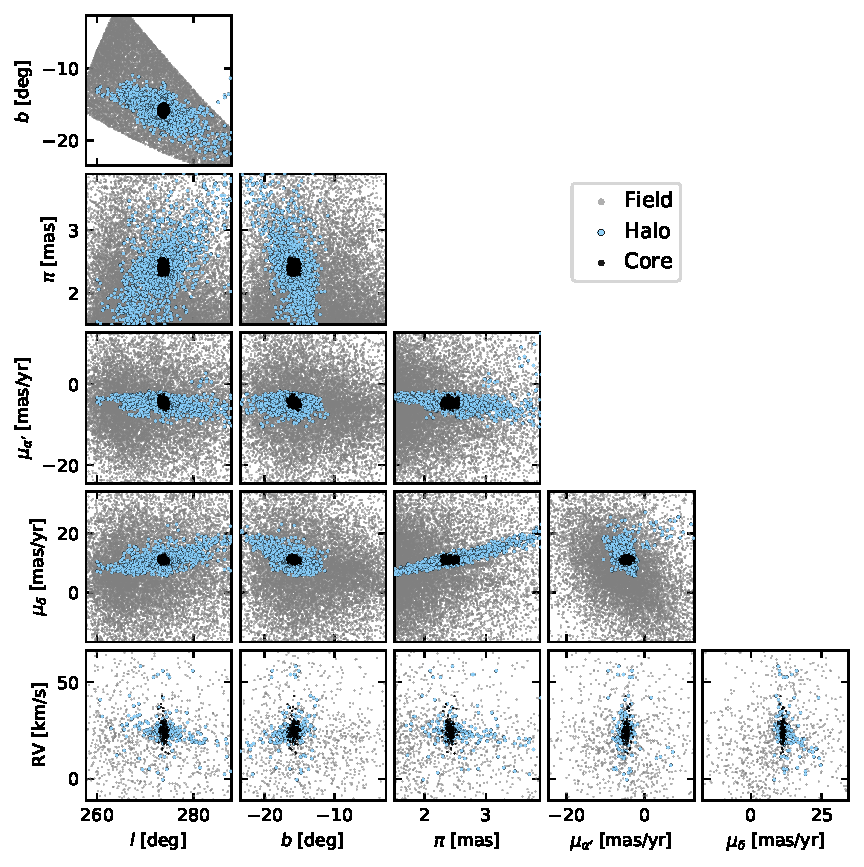
\includegraphics[width=0.95\textwidth]{f1.pdf}
	\end{center}
	\vspace{-0.7cm}
  \caption{ {\bf The dense and diffuse components of NGC\,2516 across
  position and velocity space.} The core (black) was analyzed by
  \citet{cantatgaudin_gaia_2018} using Gaia DR2, and is coincident
  with the visual overdensity of stars canonically accepted as ``the
  cluster''.  The halo (blue) is a concatenation of the studies by
  \citet{kounkel_untangling_2019} and \citet{meingast_2021}, which
  used less restrictive membership assignment algorithms described in
  Appendix~\ref{app:clustering}.  The field sample is randomly drawn
  from a $(\alpha, \delta, \pi)$ cube centered on the cluster.  The
  low volume density of the halo stars makes it difficult to visually
  distinguish the field and the halo samples.
  \label{fig:gaia6d}
	}
\end{figure*}

We selected candidate \cn\ members based on those reported in the
literature.  While a number of pre-Gaia 
studies have been performed, the
purity and accuracy of the Gaia-derived results are the current state
of the art \citep{jeffries_ngc2516_2001,Kharchenko_et_al_2013}.  We therefore adopted what we viewed as the most
interesting clustering samples to compare: those of
\citet{cantatgaudin_gaia_2018}, \citet{kounkel_untangling_2019} and
\citet{meingast_2021}.  We refer to these studies in the following as
\citetalias{cantatgaudin_gaia_2018},
\citetalias{kounkel_untangling_2019}, and \citetalias{meingast_2021}
respectively.  A useful visualization of the different samples is
available online\footnote{
  \url{https://homepage.univie.ac.at/stefan.meingast/coronae.html},
  made by \citet{meingast_2021}.}.  While we considered performing
our own clustering analysis using the Gaia data, such an effort would
in effect only replicate the work of these investigators.  We opt to
instead use their studies as starting points.

The Gaia clustering studies each used different selection functions,
which yielded different results.  \citetalias{cantatgaudin_gaia_2018}
considered stars brighter than $G=18$\,mag within a few degrees of the
cluster center, and reported 1106 candidate members of \cn.
\citetalias{kounkel_untangling_2019} and \citetalias{meingast_2021}
considered stars up to $\approx$1\,mag fainter, and reported 3003 and
1860 members respectively.  The unsupervised clustering techniques
that each of these studies applied to the second Gaia data release are
discussed Appendix~\ref{app:clustering}, as is the overlap between
their resulting membership samples.

Figure~\ref{fig:gaia6d} shows the cluster members reported by each
study in the space of positions, proper motions, and radial velocity
when available.  The \citetalias{cantatgaudin_gaia_2018} members are
all within a few degrees of the cluster center, while the
\citetalias{kounkel_untangling_2019} and \citetalias{meingast_2021}
members (the ``halo'') span tens of degrees. 
Inverting the parallax shows that members have been reported from
line-of-sight distances ranging from $300$ to $600\,$pc.
Stars in the upper right quadrant of the $\mu_{\alpha'}$ {\it vs.}
$\mu_\delta$ projection were reported almost entirely by
\citet{meingast_2021}.

In Figure~\ref{fig:gaia6d}, and for the remainder of the study, we
describe the \citetalias{cantatgaudin_gaia_2018} members as the
``core'' of the cluster, and any non-overlapping
\citetalias{kounkel_untangling_2019} and \citetalias{meingast_2021}
members as the ``halo''.  This defintion implies that there are
\ncore\ core members, and \nhalo\ halo members.  The distinction is
perhaps tautological, because \citetalias{cantatgaudin_gaia_2018} did
not extend their search for members out to tens of degrees from the
cluster center.  Nonetheless, the \citetalias{cantatgaudin_gaia_2018}
membership catalog is consistent with that of many previous
investigators \citep[{\it
e.g.},][]{jeffries_ngc2516_2001,Kharchenko_et_al_2013}, and is
consistent with the general {\it visual} impression that one has when
looking at \cn\ in the night sky: it appears to span
$\approx$2$^\circ$, not $\approx20^\circ$.

The discrepancy between our canonical understanding of open clusters
and the possibility of a diffuse population existing around \cn\
prompted our initial interest in this analysis.  What is the true
structure of \cn?  Are the core and halo truly coeval?

Outside of the core and halo, we also define a set of nearby field
stars in the ``neighborhood'' of \cn.  Based on the observed
distribution of halo members, we drew these stars randomly from the
following ``cube'' in right ascension, declination, and parallax:
\begin{align}
  \alpha\,[\mathrm{deg}] &\in [108, 132], \\
  \delta\,[\mathrm{deg}] &\in [-76, -45], \\
  \pi\,[\mathrm{mas}] &\in [1.5, 4.0].
\end{align}
We imposed a magnitude limit of $G=19$\,mag, and ran the queries using
the \texttt{astroquery.gaia} module \citep{astroquery_2018}.  We
allowed the number of stars in the comparison sample to exceed that in
the cluster sample by a factor of $\approx$5, to ensure broad sampling
of stellar masses and evolutionary states.  We also required the
comparison sample to not overlap with the cluster sample, which led to
the omission of 1.1\% of the stars drawn from the volume noted above.


\section{Age-Dating the Halo of NGC\,2516}
\label{sec:agedate}

\subsection{HR Diagram from Gaia}
\label{subsec:hr}

\begin{figure*}[t]
	\begin{center}
		\leavevmode
			%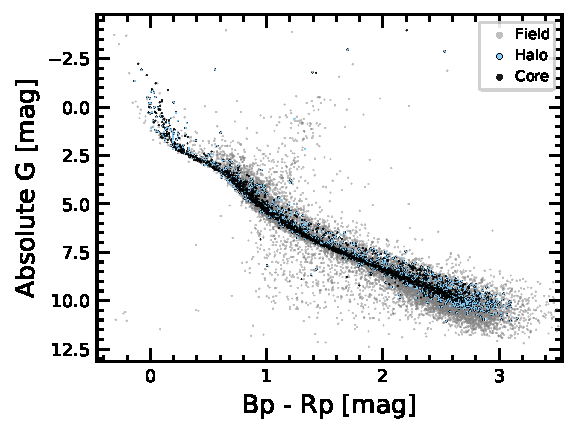
\includegraphics[width=0.85\textwidth]{f2a.pdf}
		\subfloat{
			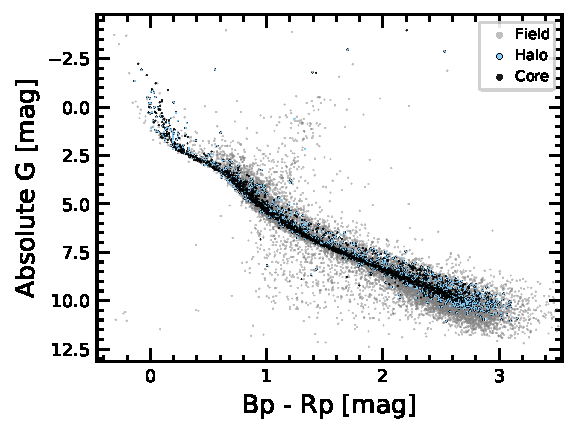
\includegraphics[width=0.49\textwidth]{f2a.pdf}
			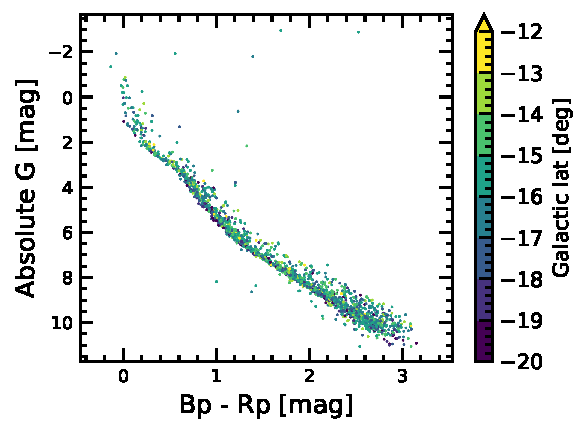
\includegraphics[width=0.49\textwidth]{f2b.pdf}
		}
	\end{center}
	\vspace{-0.7cm}
  \caption{ {\bf HR diagrams of NGC\,2516.}
    {\it Left}: Photometric data from Gaia EDR3; no reddening correction
    has been applied.  The core (black) shows a main-sequence and
    turnoff consistent with stars of a fixed age and metallicity.  The
    halo (blue) is similar, though the binary sequence is less
    defined.  At fixed color, the faintest M dwarfs in the core and
    halo are brighter than in the field star comparison sample (gray),
    consistent with these stars not having yet reached the
    main-sequence.
    {\it Right}: PARSEC isochrones ([Fe/H]=+0.06) are overplotted
    at intervals of $\log_{10}(t/\mathrm{yr})=\{8, 8.25, 8.5\}$.
    The arrow represents the average reddening correction applied
    to the models.
     The models diverge
    from the data for $M_\star \lesssim 0.45M_\odot$ ($\approx$M2V;
    $Bp-Rp\approx$2.2).
    \label{fig:hr}
  }
\end{figure*}

The first check on the plausibility of the candidate cluster members
being coeval is to analyze the Gaia Hertzsprung-Russell (HR) diagrams.  Comparable analyses
have already been performed by \citetalias{cantatgaudin_gaia_2018},
\citetalias{kounkel_untangling_2019}, and \citetalias{meingast_2021}.

Figure~\ref{fig:hr} shows the HR diagram in the space of absolute Gaia
$G$ magnitude as a function of observed $Bp-Rp$ color.  The core
members of the cluster show a clean sequence consistent with stars
with a fixed age and metallicity, and varying mass.  The halo members
mostly show a consistent main-sequence that has somewhat greater
scatter.  One possible explanation for the additional scatter could be
that the halo is more contaminated by field stars.  For instance,
$\approx5$ evolved halo stars are visible in the field-star portion of
the red giant branch (RGB).  Given the age of the system, these stars
must be field interlopers.

A separate possible explanation for scatter in the halo's HR diagram
could be differential reddening across different sightlines.  The
reported halo spans 20$^\circ$ on-sky, and varies in position from
about $b=-12^\circ$ to $b=-20^\circ$, with the stars closest to the
galactic plane also being further from the Sun by up to 300\,pc
(Figure~\ref{fig:gaia6d}).  Some empirical evidence for differential
reddening is discussed in Appendix~\ref{app:diffred}. Based on the
available evidence, we expect that both field star contamination and
differential reddening could play a role in the larger scatter of the
halo relative to the core.  A third possibility that we have not
explored is whether the binary fraction could also differ between the
different regions of the cluster.

In the right panel of Figure~\ref{fig:hr}, we compare the observed
Gaia EDR3 photometry with PARSEC isochrones
\citep{bressan_parsec_2012,chen_improving_2014,chen_parsec_2015,marigo_new_2017}.
We used the web
interface\footnote{\url{http://stev.oapd.inaf.it/cgi-bin/cmd},
\texttt{2021-02-26}, \texttt{CMD3.4}, \texttt{YBC} bolometric
corrections as in \citet{chen_2019_YBC}.} to interpolate these
isochrones at $\log_{10}(t/\mathrm{yr})=\{8, 8.25, 8.5\}$.

To determine the reddening correction across the NGC\,2516 cluster, we
queried the 2MASS
DUST
service\footnote{
	\url{http://irsa.ipac.caltech.edu/applications/DUST};
	query performed using the \texttt{astrobase.services.dust} module
	\citep{bhatti_astrobase_2018}.
}
and retrieved the extinction parameters at the positions of each
NGC\,2516 member.  The mean and standard
deviation of the $E(B-V)$ values for the \citet{schlegel_maps_1998}
and \citet{schlafly_measuring_2011} maps were consistent, so we
adopted the average from \citet{schlegel_maps_1998}: $E(B-V)_{\rm
S}=0.206\pm0.039$.  \citet{bonifacio_search_2000} found however that
the \citet{schlegel_maps_1998} maps overestimate the reddening values
when the color excess exceeds about 0.10\,mag. Applying the correction
proposed by \citet{bonifacio_search_2000} leads to our adopted
$E(B-V)=0.102\pm0.019$.  Finally, to convert to Gaia colors we used
the calibration of \citet{stassun_TIC8_2019}, namely $E(Bp-Rp)=1.31
E(B-V)$ and $A_G=2.72 E(B-V)$.  This yielded $E(Bp-Rp)=0.134\pm0.025$,
which is used in the plots.  To redden the isochrones, we assumed
$R_V=3.1$, and applied the \citet{odonnell_1994} SED-dependent
extinction law star-by-star through the PARSEC interface. 

For the metallicity, we considered a range of super and sub-solar
metallicities to fit as much of the locus from $0.5<Bp-Rp<1.5$ as
possible, and settled on the slightly super-solar $[M/H]=0.06$
\citep{cummings_2011_li_iron}.  Sub-solar metallicities led to model
predictions too blue along the main sequence by $\approx$0.1\,mag.
Our adopted metallicity agrees with the spectroscopic metallicity from
\citet[][Sec~4.4.4]{cummings_2011_li_iron}, and with the iron
abundance recently determined by the Gaia-ESO team
\citep{baratella_gaiaeso_2020}, which represented an up-revision from
an earlier sub-solar metallicity \citep{randich_gaiaeso_2018}.  While
\citet{bailey_rv_2018} report a slightly sub-solar metallicity for the
cluster, we prefer super-solar based on the goodness of fit from the
photometry.

Overall, the data and models agree for masses above approximately
0.45\,$M_\odot$.  However below this mass, the data and models diverge
at colors redder than $Bp-Rp\approx2.2$, in the sense that the model
isochrones have lower luminosities and bluer colors than the
observations.  The MIST isochrones showed a comparable disagreement
\citep{choi_mesa_2016}.  Explanations invoking both starspots and
incomplete molecular line lists have been proposed \citep[{\it
e.g.},][]{stauffer_why_2003,feiden_magnetic_2013,rajpurohit_effective_2013,mann_spectrothermometry_2013,choi_mesa_2016}.
We adopt the PARSEC isochrones since they diverge at slightly lower
mass than the MIST models, due to the temperature-opacity calibration
implemented by \citet{chen_improving_2014}.  For purposes of
age-dating the cluster, we prefer to focus on the main-sequence
turn-off (MSTO), since this is where the models have maximal predictive
power.

\citet{cummings_2018} presented techniques for mitigating some of the
complexities of MSTO age-dating ({\it e.g.}, sparse turnoffs, stellar
rotation, high binarity fractions, and the presence of blue
stragglers).  Combining a $UBV$ color-color analysis with Gaia DR2
cluster memberships, they found MSTO ages for NGC\,2516 ranging from
165 to 195\,Myr, depending on the choice of model isochrone (Y$^2$,
PARSEC, MIST, or SYCLIST).  The statistical uncertainties ($\approx
25$\,Myr) were comparable to the systematic uncertainties.

Our primary goal is to determine whether the ages of the core and halo
are consistent.  The left panel of Figure~\ref{fig:hr} suggests that
they are: stars past the turnoff in both the halo and core are on a
consistent locus.  The right panel of Figure~\ref{fig:hr} demonstrates
the precision with which the claim can be made.  The MSTO stars are
consistent with the 178 and 316 Myr models, but are bluer than the 100
Myr model.  The RGB stars are consistent only with the 178 Myr
($\log_{10} t/{\rm yr} = 8.25$) model.  Based on the assumption that
the width of the MSTO can be attributed to binary stars, we are most
interested in the blue edge. This appears most compatible with the 178
Myr model.  These results are consistent with the MSTO age range of
165 to 195\,Myr found by \citet{cummings_2018}, and we refer to their
work for a more precise model-dependent comparison.
This implies an absolute age slightly older than the Pleiades
\citep[cf.][]{mermilliod_comparative_1981}.

% FIXME: do you want to do the procedure below? Seems like overkill
% given the Cummings study.

% Our photometric age-dating procedure is as follows.  We selected all
% stars in the cluster with absolute magnitudes $M_{\rm G}>5$.  We
% excluded the six\footnote{{\bf NAMES???}} halo stars that are clear
% outliers from the rest of the cluster.  Using an isochrone grid
% spanning $\log_{10}(t/\mathrm{yr})=\{7.75 -- 8.75\}$ with 0.01\,dex
% spacing, we then numerically evaluated the $\chi^2$ fit for each
% possible age.  The resulting median, 16$^{\rm th}$, and 84$^{\rm th}$
% percentiles are used as summary statstics.
% 
% % NOTE: probably asymmetric.
% The resulting MSTO photometric age for the core is $XXX\pm YYY$\,Myr.
% For the halo, it is $XXX\pm YYY$\,Myr.  Combining the two samples
% yields $XXX\pm YYY$\,Myr.  Finally, applying the same procedure to
% the field star comparison sample gives an age of $XXX\pm YYY$\,Myr.
% [nb. the procedure should be simple and general enough that you can
% apply it to the field sample, and it'll just give a broad
% distribution...]



\subsection{Rotation from TESS}
\label{subsec:tess}

\subsubsection{Cluster Star Sample}
\label{subsubsec:cluster}

\begin{figure*}[t]
	\begin{center}
		\leavevmode
		\subfloat{
			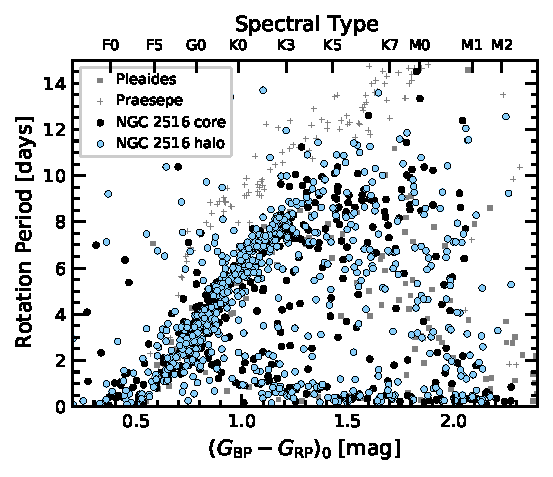
\includegraphics[width=0.49\textwidth]{f3a.pdf}
			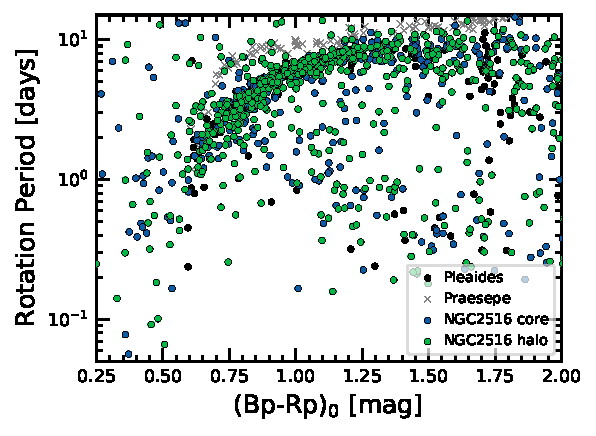
\includegraphics[width=0.49\textwidth]{f3b.pdf}
		}
	   %
		%\subfloat{
		%	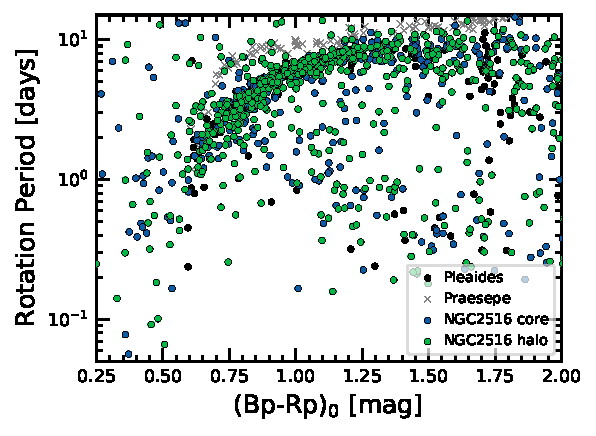
\includegraphics[width=0.6\textwidth]{f3b.pdf}
		%}
	\end{center}
	\vspace{-0.7cm}
  \caption{ {\bf The core and halo of \cn\ in the space of rotation
    period and dereddened Gaia color.}
    Subset $\mathcal{A}$ ({\it top}) and $\mathcal{B}$ ({\it bottom})
    undergo successive degrees of automated cleaning, described in Section~\ref{subsubsec:cluster}.
    The Pleiades \citep[120\,Myr;][]{rebull_rotation_2016a} and
    Praesepe \citep[650\,Myr;][]{douglas_poking_2017} are shown for
    reference.
    Stars in the core and the halo of NGC\,2516 appear
    gyrochronologically coeval with the Pleiades at $(Bp-Rp)_0$$<$1.2.
    There is a narrow range of color, from $1.2<(Bp-Rp)_0<1.7$,
    in which some NGC\,2516 members appear elevated with respect to
    the Pleiades, suggesting a slightly older age.
		\label{fig:rot}
	}
\end{figure*}

We began our rotation analysis by considering all \nkinematic\
candidate members of \cn.  For each source, we first retrieved all
available CDIPS light curves, on a per-sector basis.  This yielded
\ncdips stars with at least one sector from a CDIPS light curve, all
brighter than $Rp=16$\,mag.  \nkinematicrpltsixteen\ of the stars from
the source list have $Rp<16$.  The difference is comprised of 34 stars
unique to \citet{meingast_2021} which were not available at the time
of the CDIPS reductions and stars falling on the TESS chip gaps.  The
$Rp=16$\,mag cutoff imposed during the CDIPS processing corresponds
roughly to $(Bp-Rp)_0$ of 2.2, or a spectral type of $\approx$M2V, at
the distance of NGC\,2516.

We removed systematic trends shared between all light curves on each
CCD in each sector individually, and stitched together the resulting
light curves before searching for the periodicity.  Details regarding
our detrending approach are discussed in
Appendix~\ref{app:detrending}.  After applying the initial detrending
step aimed at removing systematic trends, we proceeding with a few
small cleaning steps aimed at improving the purity of the rotation
period measurements: we masked 0.7 days at the beginning and end of
each spacecraft orbit, and ran a sliding standard-deviation rejection
window over the light curve, which removed any outlying points within
$\pm3\times$MAD of the median in each window.

We then measured the rotation period from the resulting light curve.
We used the CDIPS aperture radius that, based on theoretical
expectations, was expected to give the optimal balance between light
from the target and background-light \citep{Sullivan_2015}.  This
typically resulted in an aperture radius of either 1 or 1.5 pixels.
To measure the periods, we used the periodogram implementations in
\texttt{astrobase}, in particular the Stellingwerf phase-dispersion
minimization periodogram, along with the more traditional Lomb-Scargle
\citep{lomb_1976,stellingwerf_period_1978,scargle_studies_1982,stellingwerf_period_2011,bhatti_astrobase_2018}.
We recorded the top five periodogram peaks from each method, and their
corresponding powers.  Finally, as a check on crowding, we also
recorded the number of stars within the aperture of equal brightness
to the target stars, and of brightness with 1.25 and 2.5 TESS
magnitudes of the target star.

Figure~\ref{fig:rot} shows the resulting rotation periods, following
three different sets of cleaning criteria.  The first and second sets
of criteria were entirely automated, and yielded subsets we denote
$\mathcal{A}$ and $\mathcal{B}$.  For both subsets, we considered
light curves for which the peak Lomb-Scargle periodogram period was
below 15 days, the normalized Lomb-Scargle power exceeded 0.08, and
for which no equal-brightness or greater companions were within the
aperture.  Beyond requiring that the target star be the brightest star
in the aperture, we also required that at most one companion with
brightness exceeding one tenth of the target star's brightness be
present in the aperture according to the Gaia DR2 source catalog.  For
set $\mathcal{A}$, this yielded \nautorotnumerator light curves,
out of \nautorotdenominator stars for which rotation periods might
plausibly have been detected.  For set $\mathcal{B}$, we
then additionally required that the Lomb-Scargle and Stellingwerf
phase-dispersion methods yielded identical periods to within 10\%.
This yielded \nautorotnumeratormatching light curves. 

The comparison to the Pleiades and Praesepe is made using the rotation
periods and dereddened colors from Table~5 of \citet{curtis_rup147_2020}, which
were based data from \citet{rebull_rotation_2016a} and
\citet{douglas_k2_2019} respectively.

A few conclusions can be drawn by comparing
the \cn\ rotation periods with those of
the Pleiades and Praesepe.
The first is that in both stages of cleaning,
the core and halo of \cn\ both show
gyrochronological ``slow sequences''.
These sequences appear to be
coeval with each other, and at least to first order
appear to overlap with the Pleiades sequence.

Second, subset
$\mathcal{A}$ is more complete than subset $\mathcal{B}$.
This completeness comes at the
expense of greater contamination.
The slow sequence
has a factor of $\sim$twice as many stars in subset
$\mathcal{A}$ than $\mathcal{B}$.
However stars above the slow sequence, which could
well be field contaminants, for the most part disappear in
subset $\mathcal{B}$.
The ``void'' underneath the slow sequence
is also more pronounced in the cleaner
subset,
though it seems to not be as empty as in
the Pleiades.

Finally, comparing the slow sequences of the Pleaides
and \cn, they appear to overlap from roughly
$0.5<(Bp-Rp)_0<1.2$.
For stars that are redder,
the dispersion in rotation periods increases.
From
$1.2<(Bp-Rp)_0<1.7$, subset
$\mathcal{B}$ of \cn\ has stars that overlap with 
the Pleiades.
However, it also has about ten stars at longer rotation periods---extending
up to $\approx$11 days, rather than the
$\approx$8.5day limit for the Pleiades.
This is consistent with \cn\ being slightly
older than the Pleiades.

{\bf We explore this quantitatively by fitting
interpolated models}[?].
The resulting gyrochronology age we find for the core is XXX.
For the halo, the claimed age from gyrochronology is YYY.
Applying the same procedure to the field star comparison sample (see
Appendix~\ref{app:compstar}),
we get an age of ZZZ+/-AAA.

\subsubsection{Kinematics $\otimes$ Rotation}

\begin{figure*}[t]
	\begin{center}
		\leavevmode
		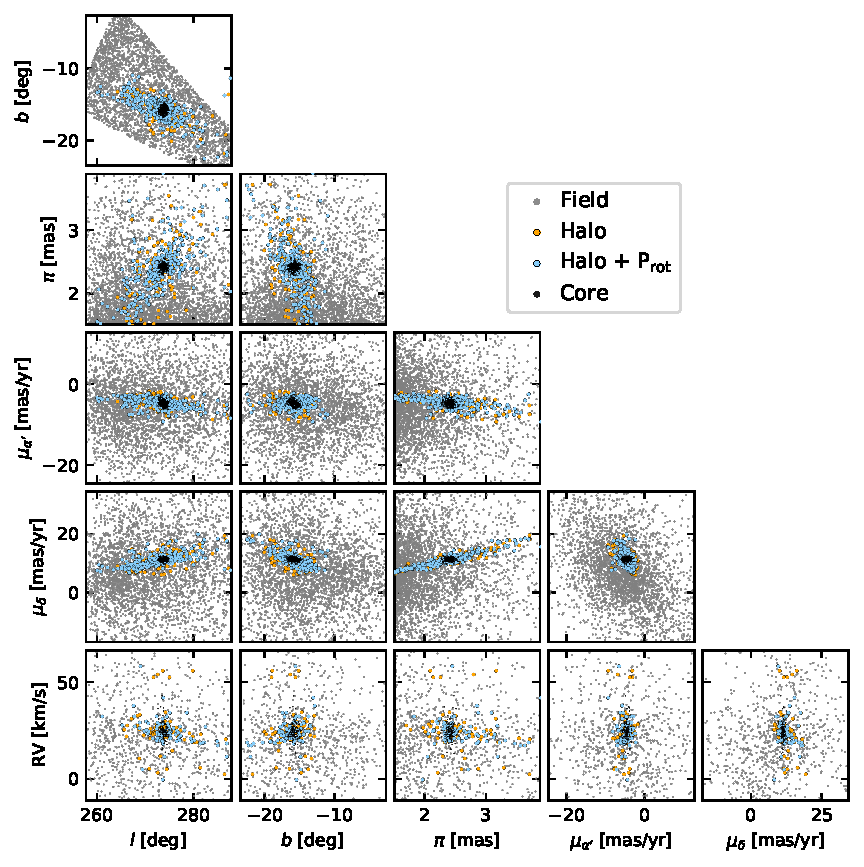
\includegraphics[width=0.95\textwidth]{f4.pdf}
	\end{center}
	\vspace{-0.7cm}
	\caption{ {\bf Gaia-based components of NGC\,2516 in position and
    velocity space, cross-matched against the rotators.}
    The plotted stars are those with $0.5<(Bp-Rp)_0<1.2$ that meet the
    crowding restrictions described in Section~\ref{subsec:tess}: they
    should have been sufficiently bright and non-crowded to enable
    rotation period detection.
		\label{fig:gaia6d_x_rotn}
	}
\end{figure*}

\begin{figure}[t]
	\begin{center}
			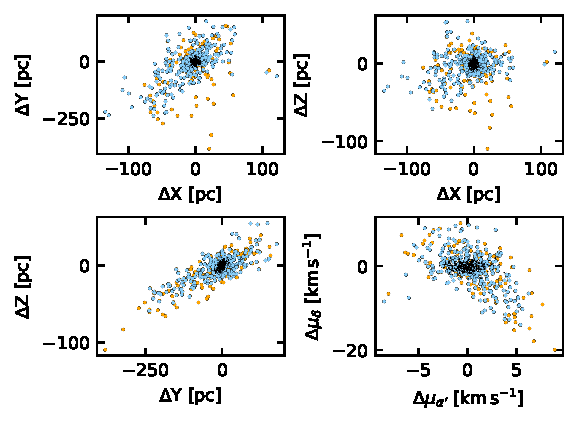
\includegraphics[width=0.49\textwidth]{f8a.pdf}
	\end{center}
	\vspace{-0.7cm}
  \caption{ {\bf Kinematic members of NGC\,2516, cross-matched against
  rotational members.}
    The projections are in galactic position coordinates and 2d-tangential velocity
    space.
    \label{fig:physical_x_rotn}
	}
\end{figure}

\begin{figure}[t]
	\begin{center}
			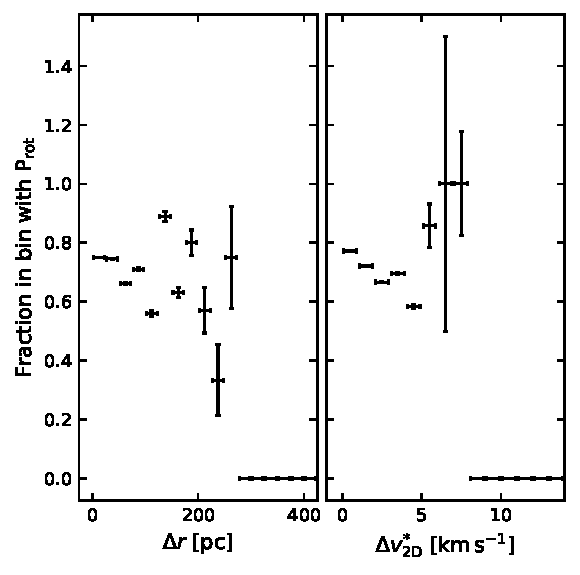
\includegraphics[width=0.49\textwidth]{f8b.pdf}
	\end{center}
	\vspace{-0.7cm}
  \caption{ {\bf Histogram of Figure~\ref{fig:physical_x_rotn}, binned
  versus 3d separation from the core and 2d velocity difference.} Bins have width
  25\,pc in position, and 2.0\,km\,s$^{-1}$ in velocity.
  {\bf Uncertainties in the fraction are taken as the quadrature sum of
  the rel unc of the numerator and denominator (FIXME)}.
  Bonafide members appear to exist hundreds of parsecs from the core, and
  up to $\approx$10\,km\,s$^{-1}$ in tangential velocity separation.
  \label{fig:hist_physical_x_rotn}
	}
\end{figure}


%\begin{figure*}[t]
%	\begin{center}
%		\leavevmode
%		\subfloat{
%			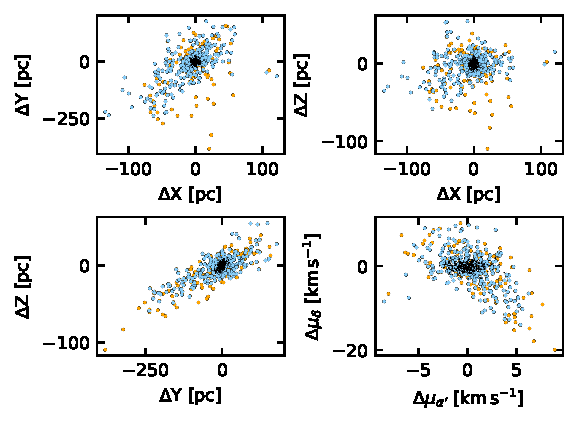
\includegraphics[width=0.75\textwidth]{f8a.pdf}
%		}
%	
%		\subfloat{
%			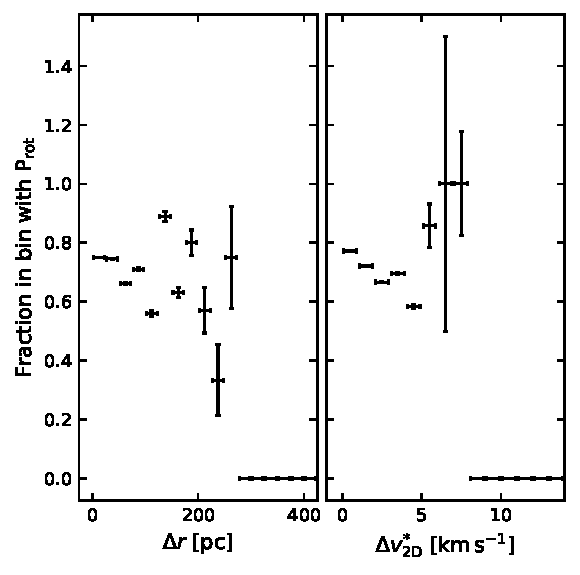
\includegraphics[width=0.75\textwidth]{f8b.pdf}
%		}
%	\end{center}
%	\vspace{-0.7cm}
%	\caption{ {\bf Gaia-based components of NGC\,2516 in position and
%    velocity space, cross-matched against the rotators, in physical
%    units.}
%    {\it Top:} projections in position and 2d-tangential velocity
%    space. {\it Bottom:} radially binned versus 3d position and
%    2d velocity difference.
%    Bins have width 25\,pc in position, and 2.0\,km\,s$^{-1}$ in
%    velocity.
%		\label{fig:physical_x_rotn}
%	}
%\end{figure*}

How far away from the core, in position and velocity space, does the
halo actually extend?  We can explore this by crossmatching the
rotator sample against \nkinematic Gaia DR2 kinematic candidate
members.  

Figure~\ref{fig:gaia6d_x_rotn} shows the result.  An important nuance
in interpreting this plot is that we show only stars with
$0.5<(Bp-Rp)_0<1.2$ for which our TESS pipeline successfully made
detrended light curves.  In other words---the base sample is the stars
for which we could have plausibly detected a rotation period.  Faint
stars with $Rp>16$ were beyond our light curve selection limit, and
crowded stars ({\it e.g.,} near saturated stars in the cluster center)
do not appear.  We selected the color limit above based on
Figure~\ref{fig:rot}, since the density of period detections seems to
decrease once $(Bp-Rp)_0 \gtrsim 1.25$, {\it i.e.}, for spectral types
later than $\approx$K4V.
Our expectation is that completion effects become important for
fainter stars.
At the distance of NGC\,2516, a K4V star has $T\approx 14.5$,
for which our reductions of the TESS images yield a precision of
$\approx 7$\,mmag per half-hour exposure \citep{bouma_wasp4b_2019}.
{\bf 
The AMPLITUDES of the rotation signals are like 10-100 mmag (CITE
REBULL 2020, FIGURE 10).
}


%G=18 is like Abs G 9.8, Bp-Rp not corrected of 2.7. 
% (Bp-Rp )_0 of 1.25 is (Bp-Rp) of 1.38... or Abs G of ~= 6.8.
% or G-Rp ~= 0.7
% So, G~=15... meaning Rp~=14.3. 

% IN POSITION
% Bin width: 25
% Rotators: [361  82  43  30  16  18  14   8   6   2   4   0   0   0   0
% 0   0   0 0   0]
% Comparison: [495 116  65  46  28  20  22  12  11   8   5   1   0   1
% 0   2   0   0 0   0]
% Rotators < 25pc : 0.72929 +/- 0.00013
% Rotators > 25pc : 0.66172 +/- 0.00023
% ... where numerator and denom are 223/337

Qualitatively, the fraction of kinematic members with TESS-detected rotation 
periods seems like it may increase with increasing distance from the halo core---both in
position and in velocity space.
To quantify this, we computed the relelvant distances in physical coordinates.
This entailed first transforming from $(\alpha, \delta, \pi)$ to galactocentric ($X,Y,Z$) which we did 
assuming the AstroPy v4.0 coordinate standard (CITE).
We then converted the on-sky proper motions to physical units by dividing by the distance of each star.
We then computed the SEPARATIONS of all of these positions and
2d-velocities from the ``median core member'', which was selected by
taking \citetalias{cantatgaudin_gaia_2018} members with membership
probability exceeding 70\%.
Again, we only considered stars for which we could have plausibly
detected a rotation period --- the same color and observability limits
discussed above were also applied.

The results are shown in Figure~\ref{fig:physical_x_rotn}.
The halo extends to separations of about 200\,pc in physical space
from the cluster core.
This corresponds to a length of $\approx$300-350\,pc, depending on
which members of the halo are chosen as the ``tips'' on either
end.

In tangential velocity space, the fraction of stars with rotation
period detections remains high out to roughly 10\,km/s.
\citet{meingast_2021} by comparison required a physically motivated
cut in tangential velocity space of 1.5 km per sec.  This probably
improves purity, but clearly doesn't get everthing for completeness.


% [361  82  43  30  16  18  14   8   6   2   4   0   0   0   0   0]
% [495 116  65  46  28  20  22  12  11   8   5   1   0   1   0   2]
% [384 109  45  27  15   4   0   0   0   0   0   0   0   0   0   0   0   0
%    0   0]
% [533 153  67  40  23  10   3   1   2   0   0   0   0   0   0   0   0   0
%    0   0]

\subsection{Lithium from Gaia-ESO and GALAH}
\label{subsec:lithium}

\begin{figure*}[t]
	\begin{center}
		\leavevmode
		\subfloat{
			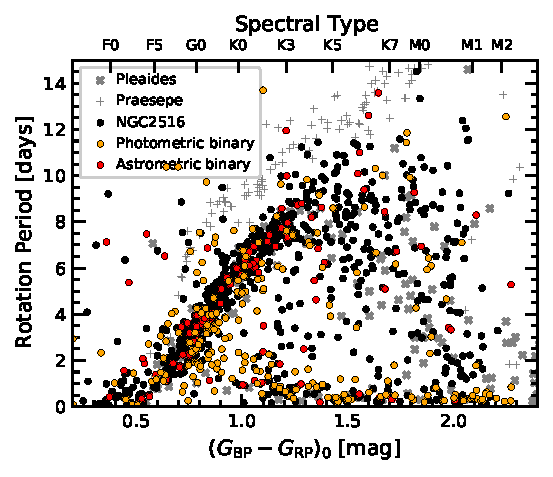
\includegraphics[width=0.75\textwidth]{f5a.pdf}
		}
	
		\subfloat{
			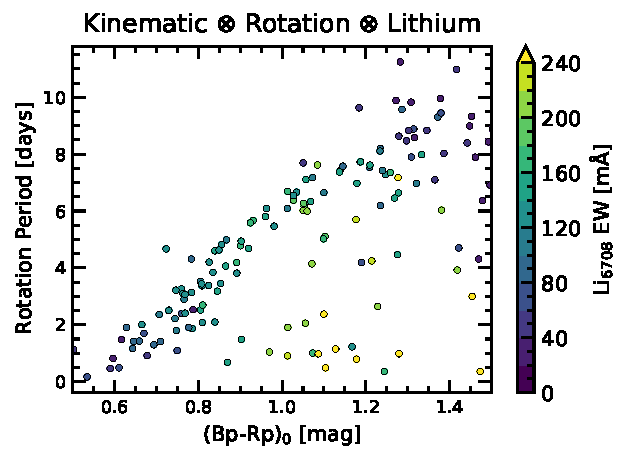
\includegraphics[width=0.75\textwidth]{f5b.pdf}
		}
	\end{center}
	\vspace{-0.7cm}
  \caption{ {\bf Lithium equivalent widths in NGC\,2516,}
  plotted against extinction-corrected color ({\it top}), and the
  combination of rotation period and extinction-corrected color ({\it
  bottom}).
  {\bf TODO: Do this against the autorot sample; Add the GALAH EWs}
  \label{fig:lithium}
  }
\end{figure*}

The third and final approach we took for age-dating the stellar
population was using the lithium deplition technique (CITE, CITE,
CITE).

Reviewing the literature, two spectroscopic datasets for \cn\ seemed
particularly important: Gaia-ESO 
\citep{randich_gaiaeso_2018} and GALAH DR3 \citep{buder_galah_2020}.
The target selection and results from each survey were as follows.

Gaia-ESO selected {\it cluster candidates} to be observed with the
GIRAFFE and UVES spectrographs based on previously reported literature
members and publicly available optical and NIR photometry.  This
target selection approach included many stars in the spatial proximity
of previously known members.  Since the possible existence of the \cn\ 
halo was not known at the time of targetting, very few ``halo'' stars
are in their ultimate sample.  For \cn, \citet{randich_gaiaeso_2018}
ultimately reported stellar parameters (including lithium equivalent
widths and metallicities) for 796 candidate members.  Cross-matching
against our kinematic list of \nkinematic candidate members by position and
imposing a 0$\farcs$5 maximum separation limit yields 492 kinematic
members for which a Gaia-ESO spectrum was acquired and stellar
parameters were reported.  15 of these (all with $(Bp-Rp)_0 > 2.0$)
are spurious matches based on the Gaia color and GES effective
temperature, and we remove them.  This yields 477 stars, of which 436
are in the core, and 41 are in the halo.  This ratio is primarily
caused by the Gaia-ESO targetting selection function.

% GALAH DR3 selected XXX/YYY.  GALAH-DR3 = GALAH-main + GALAH-faint +
% K2-HERMES + TESS-HERMES + HERMES other.  Data taken both with the 2dF
% fiber positioner, and the HERMES spectrograph at the 3.9 AAT
% (Lewis+02, Sheinis+15).  GALAH-main is 12<V<14, $\delta<+10^\circ$,
% $|b|>10^\circ$, in regions of sky with at least 400 targets in $\pi$
% square degrees (the 2dF FoV).  Fields with more than 400 targets were
% targetted multiple times, with different fiber arrangements.
% TESS-HERMES: 10.0 < V < 13.1. TESS Southern CVZ, within $12^\circ$ of
% the southern ecliptic pole.  54354 in the ``HERMES other'' program are
% from targeted observations of stars in open clusters, the GALAH Pilot
% Survey (Martell et al. 2017),

The GALAH DR3 target selection process is discussed in detail by
\citet{buder_galah_2020}.  The most relevant aspects for our project
are that the ``main'' survey targeted $12.0<V<14.0$ stars at
$\delta<+10^\circ$, provided the stars were at least ten degrees from the
galactic plane.  The survey is spatially inhomogeneous\footnote{See
the footprint at
\url{https://www.galah-survey.org/news/announcing-galah-dr3}}. Special
targeting for stars in the TESS southern continuous viewing zone, and
for known open cluster members was also performed.  We identified the
candidate \cn\ members
for which spectra had been obtained by searching
the \texttt{GALAH\_DR3\_main\_allstar\_v1} catalog, after excluding
stars with the stellar parameter bit flags 1, 2, 3.  This excludes
spectra with unreliable broadening, low S/N, and unreliable wavelength
solutions (see Table~6 of \citealt{buder_galah_2020}).  Since our main
focus is measuring equivalent widths for the Li\,6708\ \AA line, these
were the most relevant bit flags for our purpose.  Of our \nkinematic
candidate \cn\ members, 106 had spectra in GALAH DR3.  51 were in the
``core''; 55 were in the ``halo''.
77 had ``finite'' lithium, i.e., no lithium flag set.


%/Users/luke/Dropbox/proj/earhart/results/lithium/kinematic_X_galah_dr3.csv
% https://docs.datacentral.org.au/galah/dr3/catalogue-data-access/
We downloaded\footnote{Via \url{datacentral.org.au/services/download},
using the \texttt{sobject\_id} identifiers.}
the GALAH DR3 spectra for all 106 entries.
We then measured the lithium equivalent widths using PROCESS Y.
We then concatenated the GALAH DR3 and Gaia-ESO results together.

% TODO: fix the fact that the figure currently only shows Randich+18
Figure~\ref{fig:lithium} shows the results.  At fixed stellar mass
(and age), the rapid rotators tend to show elevated lithium equivalent
widths. This effect is mostly apparent in the K dwarfs.  Similar
trends in the Pleiades were noted nearly three decades ago by
\citet{soderblom_evolution_1993}.  More recent studies have found
comparable results in the Pleiades, the Psc-Eri stream, and M\,35
\citep{bouvier_pleiades_lirot_2018,arancibia_2020,jeffries_m35_li_2020}.
The fact that we see the same trend across the core and halo of \cn\ 
{\it a)} supports the conclusion that the halo is coeval with the
core, and {\it b)} suggests that the lithium-rotation correlation is
not explained by environmental effects such as the density of the cluster
during its embedded phase, but is instead tied to physical processes
acting on all low-mass pre-main-sequence stars.

% TODO: this paragraph more or less parrots the processes described by
% Bouvier+20. are there others? is there a better way to describe
% these?
Processes both internal and external to the star have been suggested to explain
the lithium-rotation trend (CITE see the recent review by Bouvier+20).
One explanation based in the stellar interior could be that the
convective mixing efficiency is anticorrelated with the surface
rotation (e.g., CITE Siess + Livio 1997, Baraffe+2017).  Another
possibility could be that stronger magnetic fields in the star's
interior inhibit convection (READ e.g., Ventura+98, Chabrier+07,
Somers + Pinsonneault 2014).  An external process that might also be
important is the effect of star-disk magnetic locking during the PMS
phase (CITE: magnetic braking).  Longer disk lifetimes would lead to
the star's outer convective zone being locked for longer while the
radiative core contracts.  The resulting differential rotation and
rotational mixing could drive the lithium depletion (CITE: Bouvier 08,
Eggenberger+12).
We have no preference between these possibilities---we simply note
that the \cn\ sample could be another helpful data point in
distinguishing them.



\section{Discussion}
\label{sec:discussion}

\subsection{How did the halo form?}
Another way to frame this question: should we call these stars a tidal
tail?
% TODO: read Gagne+20 on this...
The classical explanation of such a structure (e.g., Krumholz+19) is
that stars escape out of L1 and L2, and then form leading and lagging
arms due to differential rotation in the galaxy.
The leading and lagging arms of NGC\,2516's halo qualitatively
match this picture, in that they are oriented roughly toward and away
the direction of galactic rotation (CITE, Meingast21, link to their
website).

A second explanation though invokes
the idea that the cluster formed in a larger and lower-density star
formation complex, and the stars we see in the halo did not in fact
form in say the same ``clump'' as those in the cluster core.

% ``The stars in these halos could have escaped from the cores of the
% cluster, or they could be remnants of a larger and lower-density star
% formation complex that has since dispersed.''
Another possibility is {\it triggered star formation}.

One relevant connection may be to the ``Mamajek-2'' stellar group
(see Jilinski+2009).



\subsection{What is the contamination fraction in the halo? Does it change vs. location?}

\subsection{Are the ``very slow rotators'' bonafide members?}
Unsure. They are not isotropically distributed around the
cluster... so either triggered star formation (CITE, CITE), or they're
actually field stars.

\subsection{Mass differences between center and outer reaches?}

\subsection{Fast and blue rotators: are we going faster than other clusters?}

\subsection{Absolute age of NGC 2516}
Cummings \& Kalirai (2018) favor 150 Myr based on MSTO.
Godoy-Rivera+2021 favor 150 Myr... based on ...? what?
"""
Similar to Cummings et al. (2016), Cummings \& Kalirai (2018),
and Cummings et al. (2018) (see also Fritzewski et al. 2020 and Healy
\&
McCullough 2020)
"""

\subsection{Ways of doing this at different ages}
Some final discussion is warranted on the applicability of our
approach more generally.  This work starts with a kinematically
identified population, and then uses photometry (Gaia HR diagrams;
TESS rotation) and spectroscopy (GALAH and Gaia-ESO lithium) to
confirm youth in the stars.  Other approaches are also possible.

One can start with photometric criteria (e.g., Gaia HR diagram of
everything within some distance; Zari+18), or with spectroscopic
criteria (CITE Berger+18), or with combinations thereof (e.g., CITE
Zerjal 2019, 2020, Zhou's work).  
It might even be possible to start using chemical abundance signatures
(CITE, GALAHDR3?).

These paths might in certain cases succeed in identifying more
complete samples of dispersed members of young populations, since they
do not require kinematic proximity.




\section{Conclusion}
\label{sec:conclusion}

We analyzed X, Y, Z.
Our main results are as follows.
\begin{itemize}
	\item 
\end{itemize}


%%%%%%%%%%%%%%%%%%%%%%%%%%%%%%%%%%%%%%%%%%%%%%%%%%%%%%%%%%%%%%%%%%%%%%%%%%%%%%%


%\clearpage
\acknowledgements
\raggedbottom

The authors thank X and Y for fruitful discussions.
%
L.G.B. and J.H. acknowledge support by the TESS GI Program, program
NUMBER, through NASA grant NUMBER.
L.G.B. was also supported by a XXXX Fellowship from Princeton
University.
%
This study was based in part on observations at Cerro Tololo
Inter-American Observatory at NSF's NOIRLab (NOIRLab Prop. ID
2020A-0146; 2020B-NUMBER PI: L{.}~Bouma), which is managed by the
Association of Universities for Research in Astronomy (AURA) under a
cooperative agreement with the National Science Foundation.
%
ACKNOWLEDGE PFS / CAMPANAS.
%
This paper includes data collected by the TESS mission, which are
publicly available from the Mikulski Archive for Space Telescopes
(MAST).
%
Funding for the TESS mission is provided by NASA's Science Mission
directorate.
%
We thank the TESS Architects (George Ricker, Roland Vanderspek, Dave
Latham, Sara Seager, Josh Winn, Jon Jenkins) and the many TESS team
members for their efforts to make the mission a continued success.
%

%
% The Digitized Sky Survey was produced at the Space Telescope Science
% Institute under U.S. Government grant NAG W-2166.
% Figure~\ref{fig:scene} is based on photographic data obtained using
% the Oschin Schmidt Telescope on Palomar Mountain.
%

% %
% This research made use of the NASA Exoplanet Archive, which is
% operated by the California Institute of Technology, under contract
% with the National Aeronautics and Space Administration under the
% Exoplanet Exploration Program.
% %

% Resources supporting this work were provided by the NASA High-End
% Computing (HEC) Program through the NASA Advanced Supercomputing (NAS)
% Division at Ames Research Center for the production of the SPOC data
% products.
%

% A.J.\ and R.B.\ acknowledge support from project IC120009 ``Millennium
% Institute of Astrophysics (MAS)'' of the Millenium Science Initiative,
% Chilean Ministry of Economy. A.J.\ acknowledges additional support
% from FONDECYT project 1171208.  J.I.V\ acknowledges support from
% CONICYT-PFCHA/Doctorado Nacional-21191829.  R.B.\ acknowledges support
% from FONDECYT Post-doctoral Fellowship Project 3180246.
% %
% C.T.\ and C.B\ acknowledge support from Australian Research Council
% grants LE150100087, LE160100014, LE180100165, DP170103491 and
% DP190103688.
% %
% C.Z.\ is supported by a Dunlap Fellowship at the Dunlap Institute for
% Astronomy \& Astrophysics, funded through an endowment established by
% the Dunlap family and the University of Toronto.
% %
% D.D.\ acknowledges support through the TESS Guest Investigator Program
% Grant 80NSSC19K1727.
%
%
%
% %
% Based on observations obtained at the Gemini Observatory, which is
% operated by the Association of Universities for Research in Astronomy,
% Inc., under a cooperative agreement with the NSF on behalf of the
% Gemini partnership: the National Science Foundation (United States),
% National Research Council (Canada), CONICYT (Chile), Ministerio de
% Ciencia, Tecnolog\'{i}a e Innovaci\'{o}n Productiva (Argentina),
% Minist\'{e}rio da Ci\^{e}ncia, Tecnologia e Inova\c{c}\~{a}o (Brazil),
% and Korea Astronomy and Space Science Institute (Republic of Korea).
% %
% Observations in the paper made use of the High-Resolution Imaging
% instrument Zorro at Gemini-South. Zorro was funded by the NASA
% Exoplanet Exploration Program and built at the NASA Ames Research
% Center by Steve B. Howell, Nic Scott, Elliott P. Horch, and Emmett
% Quigley.
% %
% This research has made use of the VizieR catalogue access tool, CDS,
% Strasbourg, France. The original description of the VizieR service was
% published in A\&AS 143, 23.
% %
% This work has made use of data from the European Space Agency (ESA)
% mission {\it Gaia} (\url{https://www.cosmos.esa.int/gaia}), processed
% by the {\it Gaia} Data Processing and Analysis Consortium (DPAC,
% \url{https://www.cosmos.esa.int/web/gaia/dpac/consortium}). Funding
% for the DPAC has been provided by national institutions, in particular
% the institutions participating in the {\it Gaia} Multilateral
% Agreement.
%
% (Some of) The data presented herein were obtained at the W. M. Keck
% Observatory, which is operated as a scientific partnership among the
% California Institute of Technology, the University of California and
% the National Aeronautics and Space Administration. The Observatory was
% made possible by the generous financial support of the W. M. Keck
% Foundation.
% The authors wish to recognize and acknowledge the very significant
% cultural role and reverence that the summit of Maunakea has always had
% within the indigenous Hawaiian community.  We are most fortunate to
% have the opportunity to conduct observations from this mountain.
%
% \newline
%

\software{
  %\texttt{arviz} \citep{arviz_2019},
  \texttt{astrobase} \citep{bhatti_astrobase_2018},
  %\texttt{astroplan} \citep{astroplan2018},
	%\texttt{AstroImageJ} \citep{collins_astroimagej_2017},
  \texttt{astropy} \citep{astropy_2018},
  \texttt{astroquery} \citep{astroquery_2018},
  %\texttt{BATMAN} \citep{kreidberg_batman_2015},
  %\texttt{ceres} \citep{brahm_2017_ceres},
  \texttt{cdips-pipeline} \citep{bhatti_cdips-pipeline_2019},
  \texttt{corner} \citep{corner_2016},
  %\texttt{emcee} \citep{foreman-mackey_emcee_2013},
  %\texttt{exoplanet} \citep{exoplanet:exoplanet}, and its
  %dependencies \citep{exoplanet:agol20, exoplanet:kipping13, exoplanet:luger18,
  % 	exoplanet:theano},
	%\texttt{IDL Astronomy User's Library} \citep{landsman_1995},
  \texttt{IPython} \citep{perez_2007},
	%\texttt{isochrones} \citep{morton_2015_isochrones},
	%\texttt{lightkurve} \citep{lightkurve_2018},
  \texttt{matplotlib} \citep{hunter_matplotlib_2007}, 
  %\texttt{MESA} \citep{paxton_modules_2011,paxton_modules_2013,paxton_modules_2015}
  \texttt{numpy} \citep{walt_numpy_2011}, 
  \texttt{pandas} \citep{mckinney-proc-scipy-2010},
  %\texttt{pyGAM} \citep{serven_pygam_2018_1476122},
  %\texttt{PyMC3} \citep{salvatier_2016_PyMC3},
  %\texttt{radvel} \citep{fulton_radvel_2018},
  %\texttt{scikit-learn} \citep{scikit-learn},
  \texttt{scipy} \citep{jones_scipy_2001},
  %\texttt{tesscut} \citep{brasseur_astrocut_2019},
	%\texttt{VESPA} \citep{morton_efficient_2012,vespa_2015},
  %\texttt{webplotdigitzer} \citep{rohatgi_2019},
  \texttt{wotan} \citep{hippke_wotan_2019}.
}
\ 

\facilities{
 	{\it Astrometry}:
 	Gaia \citep{gaia_collaboration_gaia_2016,gaia_collaboration_gaia_2018}.
 	{\it Imaging}:
    Second Generation Digitized Sky Survey,
    SOAR~(HRCam; \citealt{tokovinin_ten_2018}).
 	%Keck:II~(NIRC2; \url{www2.keck.hawaii.edu/inst/nirc2}).
 	%Gemini:South~(Zorro; \citealt{scott_nessi_2018}.
 	{\it Spectroscopy}:
	CTIO1.5$\,$m~(CHIRON; \citealt{tokovinin_chironfiber_2013}),
  %PFS ({\bf CITE}),
  %  MPG2.2$\,$m~(FEROS; \citealt{kaufer_commissioning_1999}),
	%AAT~(Veloce; \citealt{gilbert_veloce_2018}).
 	%Keck:I~(HIRES; \citealt{vogt_hires_1994}).
 	%{\bf VLT (number), UVES and GIRAFFE} (CITE: Pasquini et al 2002)
% 	Euler1.2m~(CORALIE),
% 	ESO:3.6m~(HARPS; \citealt{mayor_setting_2003}).
 	{\it Photometry}:
%	  ASTEP:0.40$\,$m (ASTEP400),
% 	CTIO:1.0m (Y4KCam),
% 	Danish 1.54m Telescope,
%	  El Sauce:0.356$\,$m,
% 	Elizabeth 1.0m at SAAO,
% 	Euler1.2m (EulerCam),
% 	Magellan:Baade (MagIC),
% 	Max Planck:2.2m	(GROND; \citealt{greiner_grond7-channel_2008})
% 	NTT,
% 	SOAR (SOI),
 	TESS \citep{ricker_transiting_2015}.
% 	TRAPPIST \citep{jehin_trappist_2011},
% 	VLT:Antu (FORS2).
}

% \input{TOI837_phot_table.tex}
% %% \begin{deluxetable}{} command tell LaTeX how many columns
%% there are and how to align them.
\startlongtable
\begin{deluxetable}{llll}
    
%% Keep a portrait orientation

%% Over-ride the default font size
%% Use Default (12pt)
\tabletypesize{\scriptsize}

%% Use \tablewidth{?pt} to over-ride the default table width.
%% If you are unhappy with the default look at the end of the
%% *.log file to see what the default was set at before adjusting
%% this value.

%% This is the title of the table.
\tablecaption{\tn\ radial velocities.}
\label{tab:rvs}

%% This command over-rides LaTeX's natural table count
%% and replaces it with this number.  LaTeX will increment 
%% all other tables after this table based on this number
%\tablenum{4}

%% The \tablehead gives provides the column headers.  It
%% is currently set up so that the column labels are on the
%% top line and the units surrounded by ()s are in the 
%% bottom line.  You may add more header information by writing
%% another line between these lines. For each column that requries
%% extra information be sure to include a \colhead{text} command
%% and remember to end any extra lines with \\ and include the 
%% correct number of &s.
\tablehead{
  \colhead{Time [BJD$_\mathrm{TDB}$]} &
  \colhead{RV [m$\,$s$^{-1}$]} &
  \colhead{$\sigma_{\rm RV}$ [m$\,$s$^{-1}$]} & 
  \colhead{Instrument}
}

%% All data must appear between the \startdata and \enddata commands
% Source:
% /Users/luke/Dropbox/proj/timmy/results/paper_tables/TOI837_rv_data.tex
\startdata
 8669.533150 &  -57.8 &    27.5 &   FEROS \\
 8669.540450 &  -13.9 &    29.4 &   FEROS \\
 8676.506930 &    6.7 &    37.8 &   FEROS \\
 8677.519150 &  -70.3 &    44.6 &   FEROS \\
 8884.787630 &  240.0 &    28.0 &  CHIRON \\
 8891.891180 &  -76.0 &    37.0 &  CHIRON \\
 8898.735330 &  -10.0 &    43.0 &  CHIRON \\
 8903.725760 &  -25.0 &    38.0 &  CHIRON \\
 8904.739930 &   80.1 &    24.5 &   FEROS \\
 8905.793630 &   88.0 &    21.7 &   FEROS \\
 8908.762520 &   45.3 &    28.3 &   FEROS \\
 8909.702140 &    0.0 &    31.8 &   FEROS \\
 8912.606750 &   41.3 &    24.1 &   FEROS \\
 8913.740580 &  161.1 &    37.3 &   FEROS \\
 8915.762170 &   10.0 &    33.0 &  CHIRON \\
 8916.714540 &  -93.5 &    33.6 &   FEROS \\
 8917.765720 & -159.7 &    24.8 &   FEROS \\
 8920.706100 &   99.0 &    32.0 &  CHIRON \\
 8922.845800 & -148.3 &    54.9 &   FEROS \\
 8915.924027 &   37.5 &   725.9 &  Veloce \\
 8921.284950 &  105.9 &   453.2 &  Veloce \\
 8922.733572 & -195.9 &   195.6 &  Veloce \\
 8924.583708 &   -7.6 &   262.3 &  Veloce \\
 8926.365810 &   14.3 &   442.6 &  Veloce \\
 8927.318146 &  207.0 &   505.2 &  Veloce \\
 8928.559780 &   -7.3 &   180.2 &  Veloce \\
 8930.324059 &   -2.6 &   152.0 &  Veloce \\
 8931.293091 &  -45.7 &   152.9 &  Veloce \\
 8932.065206 & -105.6 &   319.8 &  Veloce \\
\enddata

%% Include any \tablenotetext{key}{text}, \tablerefs{ref list},
%% or \tablecomments{text} between the \enddata and 
%% \end{deluxetable} commands

%% General table comment marker
\tablecomments{
Times are in units of ${\rm BJD}_{\rm TDB} - 2{,}450{,}000$.
}
\vspace{-0.9cm}
\end{deluxetable}

% \input{ic2602_ages.tex}
% \begin{table*}
\scriptsize
\setlength{\tabcolsep}{2pt}
\centering
\caption{Literature and Measured Properties for TOI$\,$1937A}
\label{tab:starparams}
%\tablenum{2}
\begin{tabular}{llcc}
  \hline
  \hline
Other identifiers\dotfill & \\
\multicolumn{3}{c}{TIC 268301217} \\
\multicolumn{3}{c}{GAIADR2 5489726768531119616} \\
\multicolumn{3}{c}{GAIAEDR3 5489726768531119616} \\
\hline
\hline
Parameter & Description & Value & Source\\
\hline 
$\alpha_{J2016.0}$\dotfill	&Right Ascension (deg)\dotfill & 116.3707 $\pm$ 0.0109& 1	\\
$\delta_{J2016.0}$\dotfill	&Declination (deg)\dotfill & -52.3833 $\pm$ 0.0097  & 1	\\
$l_{J2016.0}$\dotfill	&Galactic Longitude (deg)\dotfill & 265.3082 & 1	\\
$b_{J2016.0}$\dotfill	&Galactic Latitude (deg)\dotfill & -13.5487 & 1	\\
%\\
%$NUV$\dotfill           & GALEX $NUV$ mag.\dotfill & 13.804 $\pm$ 0.004 & 2 \\
%$FUV$\dotfill           & GALEX $FUV$ mag.\dotfill & 18.466 $\pm$ 0.056 & 2 \\
\\
%B\dotfill			&Johnson B mag.\dotfill & 11.119 $\pm$ 0.107		& 2	\\
V\dotfill			&Johnson V mag.\dotfill & 13.18 $\pm$ 0.10		& 2	\\
%$B$\tablenote{The uncertainties of the photometry have a systematic error floor applied. Even still, the global fit requires a significant scaling of the uncertainties quoted here to be consistent with our model, suggesting they are still significantly underestimated for one or more of the broad band magnitudes}\dotfill		& APASS Johnson $B$ mag.\dotfill	& 13.001 $\pm$	0.02& 2	\\
%$V$\dotfill		& APASS Johnson $V$ mag.\dotfill	& 11.808 $\pm$	0.02& 2	\\
%\\
${\rm G}$\dotfill     & Gaia $G$ mag.\dotfill     & 13.005$\pm$0.003 & 1\\
${\rm Bp}$\dotfill     & Gaia $Bp$ mag.\dotfill     & 13.417 $\pm$0.003 & 1\\
${\rm Rp}$\dotfill     & Gaia $Rp$ mag.\dotfill     & 12.421$\pm$0.004 & 1\\
${\rm T}$\dotfill     & TESS mag.\dotfill     & 12.493$\pm$0.006 & 2\\
%$u'$\dotfill        & Sloan $u'$ mag.\dotfill & 14.706 $\pm$ 0.006& 3\\
%$g'$\dotfill		& APASS Sloan $g'$ mag.\dotfill	& 12.407 $\pm$ 0.02	&  2	\\
%$r'$\dotfill		& APASS Sloan $r'$ mag.\dotfill	& 11.311 $\pm$ 0.02	&  2	\\
%$i'$\dotfill		& APASS Sloan $i'$ mag.\dotfill	& 10.927 $\pm$ 0.04 &  2	\\
%\\
J\dotfill			& 2MASS J mag.\dotfill & 11.717  $\pm$ 0.020	& 3	\\
H\dotfill			& 2MASS H mag.\dotfill & 11.324 $\pm$ 0.026	    &  3	\\
K$_{\rm S}$\dotfill			& 2MASS ${\rm K_S}$ mag.\dotfill & 11.226 $\pm$ 0.021 &  3	\\
%\\
W1\dotfill		& WISE1 mag.\dotfill & 11.135 $\pm$ 0.023 & 4	\\
W2\dotfill		& WISE2 mag.\dotfill & 11.155 $\pm$ 0.020 &  4 \\
W3\dotfill		& WISE3 mag.\dotfill & 11.160 $\pm$ 0.086& 4	\\
W4\dotfill		& WISE4 mag.\dotfill & 9.246 $\pm$ N/A &  4	\\
\\
$\pi$\dotfill & Gaia EDR3 parallax (mas) \dotfill & 2.411 $\pm$ 0.011 &  1 \\
$d$\dotfill & Distance (pc)\dotfill & $414.7 \pm 1.9$ & 1 \\
$\mu_{\alpha'}$\dotfill		& Gaia EDR3 proper motion\dotfill & -5.627 $\pm$ 0.013 & 1 \\
                    & \hspace{3pt} in RA (mas yr$^{-1}$)	&  \\
$\mu_{\delta}$\dotfill		& Gaia EDR3 proper motion\dotfill 	&  11.309 $\pm$ 0.013 &  1 \\
                    & \hspace{3pt} in DEC (mas yr$^{-1}$) &  \\
RUWE\dotfill		& Gaia EDR3 renormalized\dotfill 	&  0.908 &  1 \\
                    & \hspace{3pt} unit weight error &  \\
RV\dotfill & Gaia EDR3 systemic \hspace{9pt}\dotfill  & $17.44 \pm 0.64$$^{\dagger}$ & 1 \\
                    & \hspace{3pt} radial velocity (\kms)  & \\
RV\dotfill & Adopted systemic \hspace{9pt}\dotfill  & $17.44 \pm 0.64$$^{\dagger}$ & 1 \\
                    & \hspace{3pt} radial velocity (\kms)  & \\
%
\\
$v\sin{i_\star}$\dotfill &  Rotational velocity (\kms) \hspace{9pt}\dotfill &  -- $\pm$ -- & 5 \\
$v_{\rm mac}$\dotfill &  Macroturbulence velocity (\kms) \hspace{9pt}\dotfill &  -- $\pm$ -- & 5 \\
${\rm [Fe/H]}$\dotfill &   Metallicity \hspace{9pt}\dotfill & -- $\pm$ -- & 5 \\
$T_{\rm eff}$\dotfill &  Effective Temperature (K) \hspace{9pt}\dotfill & ---- $\pm$ --- &  6  \\
$\log{g_{\star}}$\dotfill &  Surface Gravity (cgs)\hspace{9pt}\dotfill &  x.xxx $\pm$ 0.049  &  6 \\
%
Li EW\dotfill & 6708\AA\ Equiv{.} Width (m\AA) \dotfill & $<30$  & 7 \\
%
$P_{\rm rot}$\dotfill & Rotation period (d)\dotfill & $6.5\pm X.X$  & 8 \\
Age & Adopted stellar age (Myr)\dotfill & ---  &  9 \\
% $E(B-V)$\dotfill & Reddening (mag)\dotfill & $0.06 \pm 0.02$ & 9 \\
%
Spec. Type\dotfill & Spectral Type\dotfill & 	G2V & 5 \\
%
$R_\star$\dotfill & Stellar radius ($R_\odot$)\dotfill & X.XXX$\pm$X.XXX & 6 \\
$M_\star$\dotfill & Stellar mass ($R_\odot$)\dotfill & 1.XXX$\pm$X.XXX & 6 \\
%$F_{\rm bol}$\dotfill & Stellar bolometric flux (cgs)\dotfill & (1.967$\pm$0.046)$\times10^{-9}$ & 9 \\
$A_{\rm V}$\dotfill & Interstellar reddening (mag)\dotfill & 0.XX$\pm$0.XX & 10 \\
% $U^{*}$\dotfill & Space Velocity (\kms)\dotfill & $26.24 \pm 0.46$  & \S\ref{sec:uvw} \\
% $V$\dotfill       & Space Velocity (\kms)\dotfill & $-71.52 \pm 1.68$ & \S\ref{sec:uvw} \\
% $W$\dotfill       & Space Velocity (\kms)\dotfill & $ -1.31 \pm 0.27$ & \S\ref{sec:uvw} \\
\hline
\end{tabular}
\begin{flushleft}
 \footnotesize{ \textsc{NOTE}---
$\dagger$ Systemic RV uncertainty is the standard deviation of single-transit radial velocities, as quoted in Gaia DR2. %$*$ $U$ is in the direction of the Galactic center. \\
  {\bf FIXME}
Provenances are:
$^1$\citet{gaia_collaboration_gaia_2018},
$^2$\citet{stassun_TIC8_2019},
$^3$\citet{skrutskie_tmass_2006},
$^4$\citet{wright_WISE_2010},
$^5$CHIRON spectra,
$^6$Method~2 (cluster isochrone, Section~\ref{subsec:starparams}),
$^7$FEROS spectra,
$^8$TESS light curve,
$^9$IC~2602 ages from isochrone \& lithium depletion analyses (Section~\ref{subsec:clusterchar}),
$^{10}$Method~1 (photometric SED fit, Section~\ref{subsec:starparams}).}
\end{flushleft}
\vspace{-0.5cm}
\end{table*}

% \begin{table*}
\scriptsize
\setlength{\tabcolsep}{2pt}
\centering
\caption{Literature and Measured Properties for TOI$\,$1937B}
\label{tab:compparams}
%\tablenum{2}
\begin{tabular}{llcc}
  \hline
  \hline
Other identifiers\dotfill & \\
\multicolumn{3}{c}{TIC 766593811} \\
\multicolumn{3}{c}{GAIADR2 5489726768531118848} \\
\multicolumn{3}{c}{GAIAEDR3 5489726768531118848} \\
\hline
\hline
Parameter & Description & Value & Source\\
\hline 
$\alpha_{J2016.0}$\dotfill	&Right Ascension (deg)\dotfill & 116.3706 $\pm$ 0.0098& 1	\\
$\delta_{J2016.0}$\dotfill	&Declination (deg)\dotfill & -52.3826 $\pm$ 0.0753  & 1	\\
% $l_{J2015.5}$\dotfill	&Galactic Longitude (deg)\dotfill & 265.3082 & 1	\\
% $b_{J2015.5}$\dotfill	&Galactic Latitude (deg)\dotfill & -13.5487 & 1	\\
%\\
%$NUV$\dotfill           & GALEX $NUV$ mag.\dotfill & 13.804 $\pm$ 0.004 & 2 \\
%$FUV$\dotfill           & GALEX $FUV$ mag.\dotfill & 18.466 $\pm$ 0.056 & 2 \\
\\
%B\dotfill			&Johnson B mag.\dotfill & 11.119 $\pm$ 0.107		& 2	\\
%V\dotfill			&Johnson V mag.\dotfill & 13.18 $\pm$ 0.10		& 2	\\
%$B$\tablenote{The uncertainties of the photometry have a systematic error floor applied. Even still, the global fit requires a significant scaling of the uncertainties quoted here to be consistent with our model, suggesting they are still significantly underestimated for one or more of the broad band magnitudes}\dotfill		& APASS Johnson $B$ mag.\dotfill	& 13.001 $\pm$	0.02& 2	\\
%$V$\dotfill		& APASS Johnson $V$ mag.\dotfill	& 11.808 $\pm$	0.02& 2	\\
%\\
${\rm G}$\dotfill     & Gaia $G$ mag.\dotfill     & 17.653$\pm$0.003 & 1\\
${\rm Bp}$\dotfill     & Gaia $Bp$ mag.\dotfill     & 17.950 $\pm$0.098 & 1\\
${\rm Rp}$\dotfill     & Gaia $Rp$ mag.\dotfill     & 16.246 $\pm$0.015 & 1\\
${\rm T}$\dotfill     & TESS mag.\dotfill     & 16.86$\pm$0.08 & 2\\
$\Delta I_{\rm C}$\dotfill     & SOAR Cousins-I mag diff.\dotfill & 4.3$\pm$0.X & 2\\
%$u'$\dotfill        & Sloan $u'$ mag.\dotfill & 14.706 $\pm$ 0.006& 3\\
%$g'$\dotfill		& APASS Sloan $g'$ mag.\dotfill	& 12.407 $\pm$ 0.02	&  2	\\
%$r'$\dotfill		& APASS Sloan $r'$ mag.\dotfill	& 11.311 $\pm$ 0.02	&  2	\\
%$i'$\dotfill		& APASS Sloan $i'$ mag.\dotfill	& 10.927 $\pm$ 0.04 &  2	\\
%\\
% J\dotfill			& 2MASS J mag.\dotfill & 11.717  $\pm$ 0.020	& 3	\\
% H\dotfill			& 2MASS H mag.\dotfill & 11.324 $\pm$ 0.026	    &  3	\\
% K$_{\rm S}$\dotfill			& 2MASS ${\rm K_S}$ mag.\dotfill & 11.226 $\pm$ 0.021 &  3	\\
% %\\
% W1\dotfill		& WISE1 mag.\dotfill & 11.135 $\pm$ 0.023 & 4	\\
% W2\dotfill		& WISE2 mag.\dotfill & 11.155 $\pm$ 0.020 &  4 \\
% W3\dotfill		& WISE3 mag.\dotfill & 11.160 $\pm$ 0.086& 4	\\
% W4\dotfill		& WISE4 mag.\dotfill & 9.246 $\pm$ N/A &  4	\\
\\
$\pi$\dotfill & Gaia EDR3 parallax (mas) \dotfill & 2.351 $\pm$ 0.089 &  1 \\
$d$\dotfill & Distance (pc)\dotfill & $425.3 \pm 16.1$ & 1 \\
$\mu_{\alpha'}$\dotfill		& Gaia EDR3 proper motion\dotfill & -5.387 $\pm$ 0.104 & 1 \\
                    & \hspace{3pt} in RA (mas yr$^{-1}$)	&  \\
$\mu_{\delta}$\dotfill		& Gaia EDR3 proper motion\dotfill 	&  11.349 $\pm$ 0.096 &  1 \\
                    & \hspace{3pt} in DEC (mas yr$^{-1}$) &  \\
RUWE\dotfill		& Gaia EDR3 renormalized\dotfill 	&  1.120 &  1 \\
                    & \hspace{3pt} unit weight error &  \\
% RV\dotfill & Gaia EDR3 systemic \hspace{9pt}\dotfill  & $17.44 \pm 0.64$$^{\dagger}$ & 1 \\
%                     & \hspace{3pt} radial velocity (\kms)  & \\
% RV\dotfill & Adopted systemic \hspace{9pt}\dotfill  & $17.44 \pm 0.64$$^{\dagger}$ & 1 \\
%                     & \hspace{3pt} radial velocity (\kms)  & \\
%
% \\
% $v\sin{i_\star}$\dotfill &  Rotational velocity (\kms) \hspace{9pt}\dotfill &  -- $\pm$ -- & 5 \\
% $v_{\rm mac}$\dotfill &  Macroturbulence velocity (\kms) \hspace{9pt}\dotfill &  -- $\pm$ -- & 5 \\
${\rm [Fe/H]}$\dotfill &   Metallicity \hspace{9pt}\dotfill & -- $\pm$ -- & 5 \\
$T_{\rm eff}$\dotfill &  Effective Temperature (K) \hspace{9pt}\dotfill & ---- $\pm$ --- &  6  \\
$\log{g_{\star}}$\dotfill &  Surface Gravity (cgs)\hspace{9pt}\dotfill &  x.xxx $\pm$ x.xx  &  6 \\
%
Li EW\dotfill & 6708\AA\ Equiv{.} Width (m\AA) \dotfill & NaN  & 7 \\
%
$P_{\rm rot}$\dotfill & Rotation period (d)\dotfill & NaN  & 8 \\
Age & Adopted stellar age (Myr)\dotfill & ---  &  9 \\
% $E(B-V)$\dotfill & Reddening (mag)\dotfill & $0.06 \pm 0.02$ & 9 \\
%
Spec. Type\dotfill & Spectral Type\dotfill & 	M1V{\bf FIX} & 5 \\
%
$R_\star$\dotfill & Stellar radius ($R_\odot$)\dotfill & 0.XXX$\pm$X.XXX & 6 \\
$M_\star$\dotfill & Stellar mass ($R_\odot$)\dotfill & 0.XXX$\pm$X.XXX & 6 \\
%$F_{\rm bol}$\dotfill & Stellar bolometric flux (cgs)\dotfill & (1.967$\pm$0.046)$\times10^{-9}$ & 9 \\
$A_{\rm V}$\dotfill & Interstellar reddening (mag)\dotfill & 0.XX$\pm$0.XX & 10 \\
% $U^{*}$\dotfill & Space Velocity (\kms)\dotfill & $26.24 \pm 0.46$  & \S\ref{sec:uvw} \\
% $V$\dotfill       & Space Velocity (\kms)\dotfill & $-71.52 \pm 1.68$ & \S\ref{sec:uvw} \\
% $W$\dotfill       & Space Velocity (\kms)\dotfill & $ -1.31 \pm 0.27$ & \S\ref{sec:uvw} \\
\hline
\end{tabular}
\begin{flushleft}
 \footnotesize{ \textsc{NOTE}---
% $\dagger$ Systemic RV uncertainty is the standard deviation of single-transit radial velocities, as quoted in Gaia DR2. %$*$ $U$ is in the direction of the Galactic center. \\
  {\bf FIXME}
Provenances are:
$^1$\citet{gaia_collaboration_gaia_2018},
$^2$\citet{stassun_TIC8_2019},
$^3$\citet{skrutskie_tmass_2006},
$^4$\citet{wright_WISE_2010},
$^5$CHIRON spectra,
$^6$Method~2 (cluster isochrone, Section~\ref{subsec:starparams}),
$^7$FEROS spectra,
$^8$TESS light curve,
$^9$IC~2602 ages from isochrone \& lithium depletion analyses (Section~\ref{subsec:clusterchar}),
$^{10}$Method~1 (photometric SED fit, Section~\ref{subsec:starparams}).}
\end{flushleft}
\vspace{-0.5cm}
\end{table*}

% \input{model_posterior_table.tex}

\clearpage
\bibliographystyle{yahapj}                            
\bibliography{bibliography} 

\appendix
\section{Clustering methods and outcomes}
\label{app:clustering}

\begin{figure*}[h]
	\begin{center}
		\leavevmode
		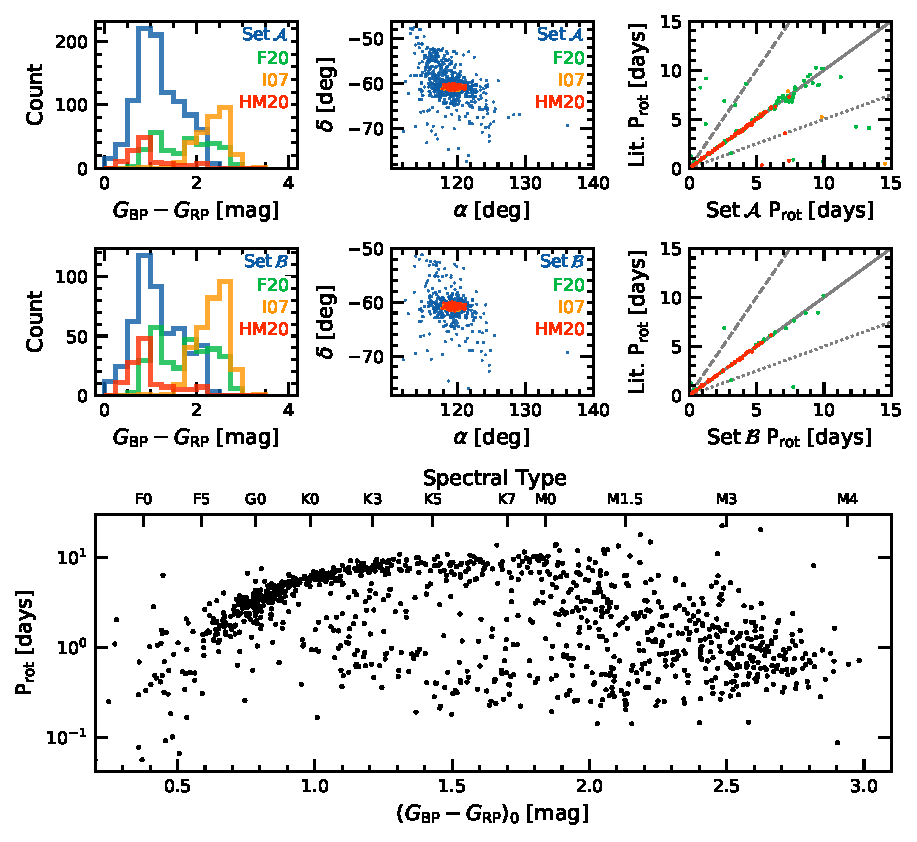
\includegraphics[width=0.4\textwidth]{f10.pdf}
	\end{center}
	\vspace{-0.7cm}
  \caption{ {\bf Different clustering techniques yield different
  outcomes.} \nkinematic unique candidate cluster members found
  using three different techniques are considered in this study.
  \citetalias{cantatgaudin_gaia_2018}: \citet{cantatgaudin_gaia_2018},
  \citetalias{kounkel_untangling_2019}:
  \citet{kounkel_untangling_2019}, \citetalias{meingast_2021}:
  \citet{meingast_2021}.
  \label{fig:venn}
	}
\end{figure*}

Figure~\ref{fig:venn} is a Venn diagram showing the overlap between
the three membership catalogs concatenated in this study.  99\% of the
\citetalias{cantatgaudin_gaia_2018} sample overlaps with
\citetalias{kounkel_untangling_2019}, \citetalias{meingast_2021}, or
both.  By comparison, 36\% of the \citetalias{kounkel_untangling_2019}
sample, and 15\% of the \citetalias{meingast_2021} sample are
non-overlapping.
The data---Gaia DR2---used by all the studies was the same.
What are the differences in methodology that produce these different
outcomes?

%
% TODO: the following two paragraphs, WHEN QUOTED, are ENTIRELY FROM
% the relevant papers. they should probably be nixed in favor of
% concision.
%
\citetalias{cantatgaudin_gaia_2018} applied a procedure that 
yielded what we call ``the core''.  Their procedure was to first query
a Gaia DR2 cone around the previously reported RA and dec of the
cluster, and within $\pm 0.5$\,mas of its previously reported
distance. 
% TODO: which was it?
The outer radius of their cone was either r2 from MWSC (CITE
Kharchenko 2013), or twice the ``cluster radius'' listed by DAML/Dias (CITE).  No
proper motion cut was applied.  They then applied an unsupervised
classification scheme called UPMASK to $G<18$\,mag stars within this
cone (CITE).  The steps of UPMASK are first to perform a k-means
clustering in the ``astrometric space'' ($\mu_{\alpha'}, \mu_\delta,
\pi$).  Then, a ``veto'' step is applied to assess whether the groups
of stars output from the k-means clustering are or are not more
concentrated than a random distribution.  This is implemented by
``comparing the total branch length of the minimum spanning tree
connecting the stars with the expected branch length for a random
uniform distribution covering the investigated field of view''.  ``To
turn this yes/no flag to a membership probability,
\citet{cantatgaudin_gaia_2018} then redraw new values of
($\mu_{\alpha'}, \mu_\delta, \pi$) for each source based on the listed
value, uncertainty, and covariance.  After a certain number of
redrawings, the final probability is the frequency with which a given
star passes the veto".  In the case of \cn, this yielded a reported
``\texttt{r50}'' within which half of the cluster members were found
to be within 0.496$^\circ$.
When we selected candidate \cn\ members from the results of
\citetalias{cantatgaudin_gaia_2018}, we opted to include all candidate members
with reported membership probability exceeding 10\%.
While this seems {\it a priori} low, our results ({\bf SECTION XXX})
show that this ``membership probabilty'' severely underestimates the
purity of the \citetalias{cantatgaudin_gaia_2018} sample for \cn. 
%TODO: quantify
Their false positive rate across the sample is more like 1-5\%.

\citetalias{kounkel_untangling_2019}
applied a different unsupervised
clustering method to the 5-dimensional Gaia DR2 data (omitting radial
velocities, due to their sparsity).  Their selection function (see
their Section~2) yielded $\approx 2\times 10^7$ stars, mostly within
$\approx 1$\,kpc and typically with $G<18$\,mag.  Their clustering
algorithm, which was run on this entire  stellar sample,
 was the ``hierarchical density-based spatial clustering of
applications with noise'' (HDBSCAN, CITE McInnes17).  The classical
DBSCAN algorithm ``identifies clusters as overdensities in a
multi-dimensional space in which the number of sources exceeds the
required minimum number of points within a neighborhood of a
particular linking length $\epsilon$.  HDBSCAN does not depend on
$\epsilon$; instead it condenses the minimum spanning tree by pruning
off the nodes that do not meet the minimum number of sources in a
cluster and reanalyzing the nodes that do. Depending on the chosen
algorithm, it would then either find the most persistent structure
(through the excess of mass method), or return clusters as the leaves
of the tree (which results in somewhat more homogeneous clusters). In
both cases it is more effective at finding structures of varying
densities in a given data set than DBSCAN.''
`` The two main parameters that control HDBSCAN are the number of
sources in a cluster and the number of samples. The former is the
parameter that rejects groupings that are too small; the latter sets
the threshold of how conservative the algorithm is in its
considerations of the background noise (even if the resulting noisy
groupings do meet the minimum cluster size).  By default, the sample
size is set to the same value as the cluster size, but it is possible
to adjust them separately.''
Regarding membership proabilities,
\citetalias{kounkel_untangling_2019} did not report continuous membership
probabilities, instead opting for the binary ``member'' or ``not''.

\citetalias{meingast_2021} did the same as
\citetalias{kounkel_untangling_2019}, but required A) the tangential
velocity dispersions to be smaller, and B) deconvolved the distances.
{\bf FIXME FIXME FIXME}
{\bf FIXME FIXME FIXME}
{\bf FIXME FIXME FIXME}

\citet{meingast_2021} reported a 
Finally, 1577 of the 1860 \citet{meingast_2021} sources (85\%)
were included in the \citet{kounkel_untangling_2019} sample.  





\section{Detrending details}
\label{app:detrending}

In ``detrending'' for our general variability search, our goal was to
preserve astrophysical variability, while removing systematic
variability.  One particular concern for the TESS light curves is
systematic variability at the timescale of the 14-day satellite orbit,
mostly induced by scattered light from the Earth and Moon.

We therefore turned to the principal components (i.e., the
eigenvectors) calculated following the procedure described by
\citet{bouma_cdipsI_2019}. In brief, these vectors are computed using
a set of ``trend stars'' selected from across each CCD according to
ad-hoc heuristics that (hopefully) lead them to be dominated by {\it
systematic} variability (Sec~3.7.2).

The principal component vectors, also referred to as the eigenvectors,
are rank-ordered by the degree of variance that they predict in the
training set (of ``trend stars'').

We then posit that any given target star's light curve is described as
a linear combination of the eigenvectors.  Optionally, we also
considered the inclusion of additional systematic vectors that could
affect the light curve, such as the CCD temperature, the flux level
measured in the background annulus, and the centroid positions of the
stars on the CCDs.  These can be treated as additional ``features'' in
the linear model.

To determine the coefficients of the linear
model after the full set of eigenvectors (plus optionally
``sytematic'' vectors) had been asssembled,  we explored two possible
methods: ordinary
least squares, and ridge regression. Ridge regression is the same as
ordinary least squares, except it includes an L2 norm with a regularization
coefficient. The regularization coefficient that best applied for any
given target light curve was solved for using a cross-validation grid
search, using \texttt{sklearn.linear\_modelRidgeCV} (CITE). 

Each target light curve was mean-subtracted and normalized by its
standard deviation, as were the eigenvectors. The linear problem was
then solved numerically, and the light curve was reconstructed by re-adding the
original mean, and re-multiplying by the standard deviation to ensure
that the variance of the light curve did not change.

We found that the choice of using ordinary
least squares versus ridge regression did not seem to significantly
affect the resulting light curves. In other words, the inclusion (or
lack thereof) of a regularization term did not strongly alter the
best-fitting coefficients.
In the spirit of ``KISS'', we opted to use ordinary least squares.

A few other choices seemed to be more important:

\begin{itemize}

  \item {\it To smooth, or to not smooth the eigenvectors}.
  Ideally, the eigenvectors should be smooth in time. They should not contain
    residuals from {\it e.g.}, eclipsing binaries that snuck their way
    into the template set, and they should also not be intrinsically noisier
    than the target star. If either of these is the case (and we found that
    it sometimes was), it can
    induce extra variability into the PCA ``detrended'' light curves.
    To address this problem, we opted to smooth the eigenvectors using
    a time-windowed filter (with a "biweight" weight scheme, implemented in
    \texttt{wotan} by \citet{hippke_wotan_2019}; window length 1 day, cval 6).
  One issue with this is that systematic sharp features (captured e.g., in
  "spike vectors") no longer are captured, so they end up in the "PCA
  detrended" light curves. They can then be filtered out
  ({\it e.g.}, using rolling outlier rejection), and we prefer this approach to having
  systematic features being {\it injected by} the PCA detrending.

  \item {\it How many eigenvectors to use}.
    A larger number always leads to greater whitening.  In
    \citet{bouma_cdipsI_2019}, we performed a Factor Analysis
    cross-validation to determine the number of eigenvectors to use.
    The typical number adopted based on this analysis was 10--15.
    While this approach should in theory prevent over-fitting, in
    our experience, for stellar rotation it still often lead to
    distorts the signals, especially for rotation signals with small amplitudes
    and periodicities of
    $\gtrsim 3$ days.  (Shorter signals typically are not distorted,
    since the eigenvectors do not contain the high-frequency
    content that leads to the distortions).  For the present analysis, we
    therefore impose the maximum number of eigenvectors to be 5.

  \item {\it Which supplementary systematics vectors to use}.
    We considered using the \texttt{BGV}, \texttt{CCDTEMP},
    \texttt{XIC}, \texttt{YIC}, and \texttt{BGV} vectors, packaged
    with the CDIPS light curves. We found that the background value
    measured in an annulus centered on the aperture, \texttt{BGV},
    tended to produce the best independent information from the PCA
    eigenvectors, and so we adopted it as our only ``supplementary''
    trend vector.  We opted to not smooth it (in hopes that it would
    provide direct complement to the smoothed PCA vectors; 1 sharp
    vector containing literally the background information, plus 5
    smooth vectors).
\end{itemize}

For every ``target star'', we then decorrelated the raw
(image-subtracted and background-subtracted) light curve
using a linear model with ordinary least squares.

\section{Comparison Star Rotation Periods}
\label{app:compstar}

\begin{figure}[t]
	\begin{center}
		\leavevmode
    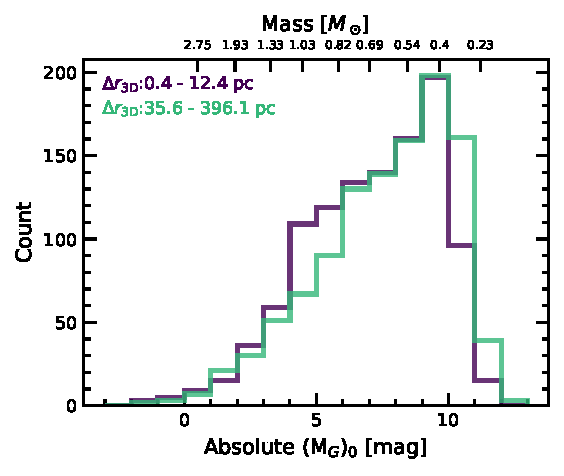
\includegraphics[width=0.49\textwidth]{f9.pdf}
	\end{center}
	\vspace{-0.7cm}
	\caption{ {\bf Rotation in NGC\,2516 compared to the field.}
  Stars with Gaia $Rp<13$\,mag in the cluster and field samples were
  considered. (Fainter stars in the field sample were not studied as part
  of the broader CDIPS project).
  The field stars show a different rotation period distribution than
  the kinematically selected NGC\,2516 members.
  \label{fig:compstar}
	}
\end{figure}

To provide a basis for comparison, we also opted to search the
``calibration'' light curves ($Rp<13$) that were created as a part of
the CDIPS project.  Over the southern sky (Sectors 1-13 of TESS), this
corresponded to a sample of \ncalibration stars.  Cross-matching these
against the \nnbhd randomly drawn stars in the neighborhood of \cn yielded
\nnbhdcalibstar unique stars, with a cumulative total of \nnbhdcaliblc TESS
sectors observed.
The magnitude cut of $Rp<13$ at the distances of the neighborhood sample
corresponds to an extinction-corrected color cutoff of $(Bp-Rp)_0
\approx 0.80$, or spectral types of $\approx$G1V.
This reaches sufficiently far down the main-sequence to enable a
comparison to the cluster star sample.

We performed the same light curve stitching and period-search
procedure on the field comparison stars.
Imposing the same requirements for crowding resulted in
\ncompstardenominator stars for which rotation periods could have been
detected.
Imposing the same Lomb Scargle power cutoff, and period upper limit,
yielded \ncompstarnumerator period detections (\ncompfrac).
Within the same brightness cutoff, 
\nautovscompstarnumerator of \nautovscompstardenominator cluster stars
yielded period detections (\nautofrac).
Though the detection fractions are frankly not very different
(likely because of the brightness cutoff), the period {\it
vs} color distributions are quite different
(Figure~\ref{fig:compstar}).





\section{Differential Reddening}
\label{app:diffred}

\begin{figure*}[t]
	\begin{center}
		\leavevmode
			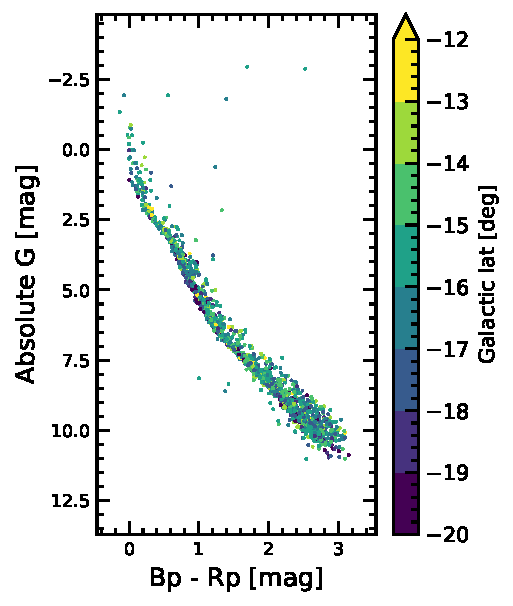
\includegraphics[width=0.75\textwidth]{f2c.pdf}
	\end{center}
	\vspace{-0.7cm}
  \caption{ {\bf HR diagram of NGC\,2516, using Gaia EDR3 photometry.}
    {\it Bottom:} Reported members of the halo, as a function of
    galactic latitude. Can the additional scatter in the halo be
    understood through differential reddening?
    {\bf Maybe}.
    \label{fig:diffred}
  }
\end{figure*}

Figure~\ref{fig:diffred}.


\section{Rotation $\otimes$ RUWE}
\label{app:ruwe}

\begin{figure*}[t]
	\begin{center}
		\leavevmode
		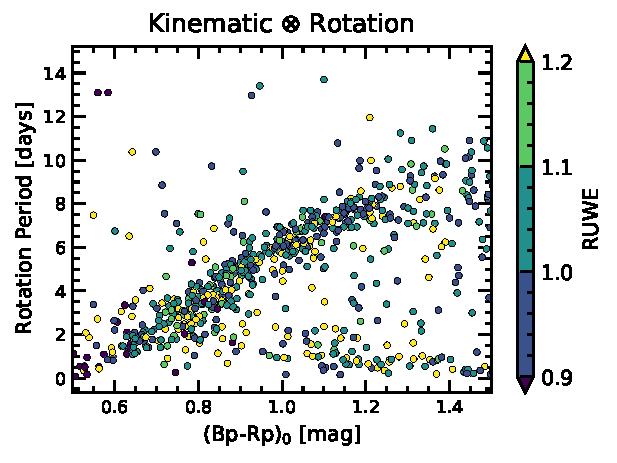
\includegraphics[width=0.95\textwidth]{f6.pdf}
	\end{center}
	\vspace{-0.7cm}
	\caption{ {\bf Rotation versus color, colored by RUWE.}
		Looks like on the slow sequence, there's more yellow at the bottom?
		\label{fig:rotn_X_RUWE}
	}
\end{figure*}

Figure~\ref{fig:rotn_X_RUWE}.


\section{Kinematics $\otimes$ Rotation in EDR3}

\begin{figure*}[t]
	\begin{center}
		\leavevmode
		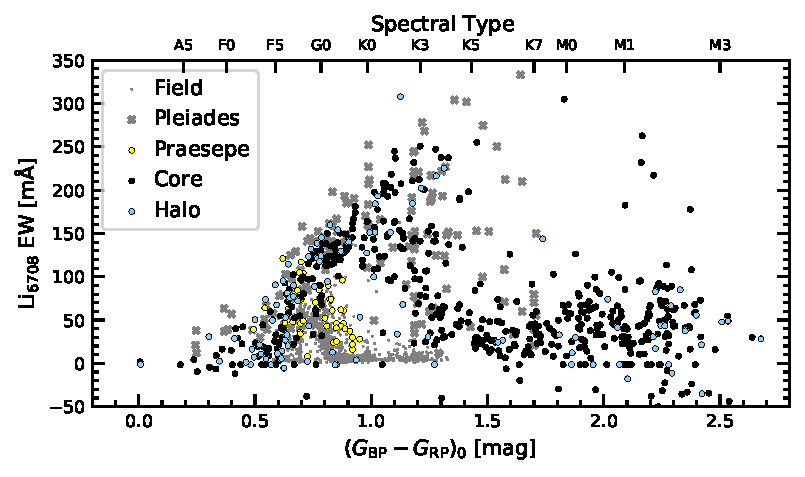
\includegraphics[width=0.95\textwidth]{f7.pdf}
	\end{center}
	\vspace{-0.7cm}
	\caption{ {\bf Gaia-based components of NGC\,2516 in position and
    velocity space, cross-matched against the rotators. Analog of
    Figure~\ref{fig:gaia6d_x_rotn}, but showing EDR3 kinematics.}
		\label{fig:gaia6d_x_rotn_EDR3}
	}
\end{figure*}

How did we do?
Figure~\ref{fig:gaia6d_x_rotn_EDR3} lets us check with a more precise
astrometric solution.






\listofchanges

%\allauthors
\end{document}
